\chapter{Analyse der Ergebnisse}

In diesem Kapitel findet man Informationen über die durchgeführten Programmtests. Ziel der Testfälle ist es zu bestimmen, wie gut meine Implementierung des ANFIS-Models lernt. In jedem Unterkapitel wird gegen eine bestimmte Eigenschaft getestet. Bei der Untersuchung nehme ich in Betrachtung zwei mathematischen Funktionen, zwar die Parabel- und Sinusfunktion. Die Tests werden anhand Variation von drei Variablen - Anzahl Fuzzymengen und Iterationen, und Gradient-Descent-Arten. 

Bei den Tests werden drei Arten von Gradient-Descent-Verfahren angesetzt - Stochastischen, Mini-Batch und Batch Gradienten Verfahren. Deren Eigenschaften werden in den nächsten Unterkapiteln erläutert. 

Außerdem werde ich zwei unterschiedlichen Berechnungsweisen für die Zugehörigkeitsfunktionen verwenden. Das Endergebnis der Funktionen ist gleich, jedoch lernt das Modell unterschiedlich. Die zwei Arten nenne ich MF-Typ 0 und MF-Typ 1. Wenn ich vom MF-Typ 0, oder nur Typ 0, spreche, meine ich, dass die Zugehörigkeitsberechnung in zwei Teilen untergegliedert ist. Man kann das Dreieck, das durch die drei Parametern der Zugehörigkeitsfunktion bestimmt ist, durch die Mitte teilen. Dann entstehen zwei Bereiche, die separat betrachtet werden. Auf dieser Weise entstehen zwei Gleichungen (Teilen). Bei dem Typ 1 erfolgt die Berechnung in einer Gleichung. Also da wird nicht unterschieden, wo der X-Wert auf der Hypothenuse liegt - kleiner oder größer als der Mittelpunkt. Die zwei Berechnungsweisen für MF-Typ 0 \ref{mf_typ0} und MF-Typ 1 \ref{mf_typ1} gebe ich als Gesammtformel an.
\begin{align}
	\begin{split}\label{mf_typ0}
		\mu(x) = \max[\min(\frac{x - a}{m - a}, \frac{b - x}{b - m}), 0.0]
	\end{split}\\
	\begin{split}\label{mf_typ1} 
		\mu(x) = \max[0, 1 - 2\frac{\lvert x - m\rvert}{b - a}]
	\end{split} 
\end{align}
%H. Bothe, Neuro-Fuzzy-Methoden zweite Gleichung
Die erste Berechung ist von MF-Typ 0 und die Zweite von Typ 1. In der Gleichung sind die Größen \textit{a, m und b} die Parametern der Zugehörigkeitsfunktion. Die Variable \textit{a und b} sind die zwei Grenzwerte entsprechend links und rechts, und \textit{m} ist der Gipfelpunkt, oder Mittelpunkt.

Alle unseren Lerndaten werden aus einer Datei, die einen spezifischen Aufbau hat, gelesen. Die Daten können in zwei Gruppen aufgeteilt werden - Eingaben und Soll-Ergebnisse. Jede Spalte beinhaltet Elemente aus einer der beiden Gruppen, wobei die Letzte immer die Soll-Ergebnisse enthält. Da in diesem Projekt einstellige Funktionen in betracht genommen werden, gibt es in der Datei nur zwei Spalten.

Nachdem alle Verfahren vorgestellt wurden, wird mit den Tests begonnen.Wegen der größe Anzahl an Tests werden nur bestimmte ausgewählt. Eine Tabelle und alle Modellgrafiken werden später am Ende der Ausarbeitung angehängt. 

Die Vorgehensweise bei der Beschriftung der Testfälle erfolgt für beide Funktionen gleich. Für ein Model wird seine Struktur und seine Eigenschaften gegeben. Weiterhin wird das Ergebnisgrafik gezeichnet. Zum Schluss werden die gelernten Konklusionsfunktionen vorgestellt. Zu jedem Teil wird eine Erläuterung zusätzlich aufgeführt. 
 
\subsubsection{Stochastic Gradient Descent}
Bei dem stochastischen gradienten Verfahren (Stochastic Gradient Descent) handelt es sich um eine spezifische Eingabenweise. Bei dieser Vorgehensweise werden einzelnen Einträgen aus dem Datensatz als Eingabe in das Model gegeben. Somit beschreibt ein Element eine Iteration (Epoche) in dem Lernprozess. Nach jeder Iterationen werden die betroffenen Gewichten (Parametern) angepasst. Dieses Verfahren wird am seltesten von Allen (Stochastic, Mini-Batch und Batch) eingesetzt.


\subsubsection{Mini-Batch Gradient Descent} \label{mini_batch}
Bei dem Mini-Batch Verfahren werden kleine Sets, normalerweise zwischen 30 und 500 Elemente, aus der Menge der Daten genommen und diese an dem Model zum Lernen gegeben. Das heißt eine Iterationen wird erst dann durchgeführt, wenn alle Elemente aus dem Batch abgearbeitet werden. Dieses Verfahren wird öfters bei Lernaufgaben verwendet, bei dennen der Datensatz extrem groß ist. In meinem Programm baue ich Zufälligkeit, sodass die Lernmenge zufällig aus der Gesamtmenge auszuwählen ist.

\subsubsection{Batch Gradient Descent}\label{batch}
Bei dem Batch Gradient Descent setzt man eine Architektur, bei der alle Daten in dem Lernprozess innerhalb eines Lernzugs fließen. Diese Art ist gut geeignet, bei Problemstellungen, wo die Datenbasis angemessen groß ist. In unseren zwei Fällen handelt es sich um relativ kleine Datenmengen (400 und 1000 Datensätze entsprechend für Sinus- und Parabelfunktion). Bei Lernaufgaben mit 100 Tausende von Datensätze ist diese Vorgehensweise ungeeignet. Da ist das Mini-Batch-Verfahren einzusetzen.

\section{Lernen der Sinusfunktion mit Stochastic Gradient Descent}
In diesem Kapitel wird die Sinusfunktion untersucht. Hier erläutere ich die Ergebnisse, die bei den Lernvorgängen erschaffen wurden. Zum Schluss verschaffe ich einen Überblick über die besten Eigenschaften zum Lernen der Sinusfunktion.

Die Sinusfunktion ist als Zeichnung (siehe \ref{sinus}) angegeben.

\begin{figure}
	\centering
	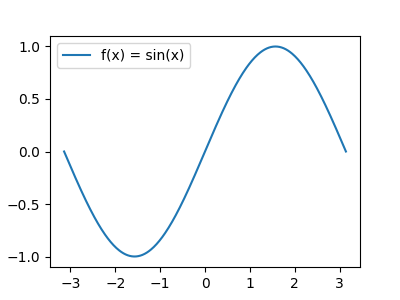
\includegraphics{images/sinus.png}
	\caption{Die  Sinusfunktion.}
	\label{sinus}
\end{figure} 

\subsubsection{Lernen eines Models mit 2 Fuzzy Sets und 1 Ablauf}

Anfangend lasse ich das Model einen Lauf durchführen. Wobei hier wichtig zu erwähnen ist, dass eine Iteration und ein Lauf nicht das selbe ist. Iteration im stochastischen Verfahren bedeutet, dass ein Element aus der Datenmenge verarbeitet wurde und ein Lauf - dass alle Elemente erarbeitet sind. Also heißt es für unsere Laufzeit, dass das Model bereits nach einem Lauf 400 Iterationen ausgeführt hat. Die 400 Epochen haben ca. 1.16s gebraucht, wenn wir MF-Typ 0 verwenden. Bei dem MF-Typ 2 werden etwa 0.3s gespart - ca. 0.86s Lerndauer. Die Ergebnisse aus beiden Lerngänge werden unten in zwei Grafiken (\ref{2Sets400_Stoch_0} und \ref{2Sets400_Stoch_1}) zuerst und dann Daten in einer Tabelle gegeben.

\begin{figure}[htbp]
	\centering
	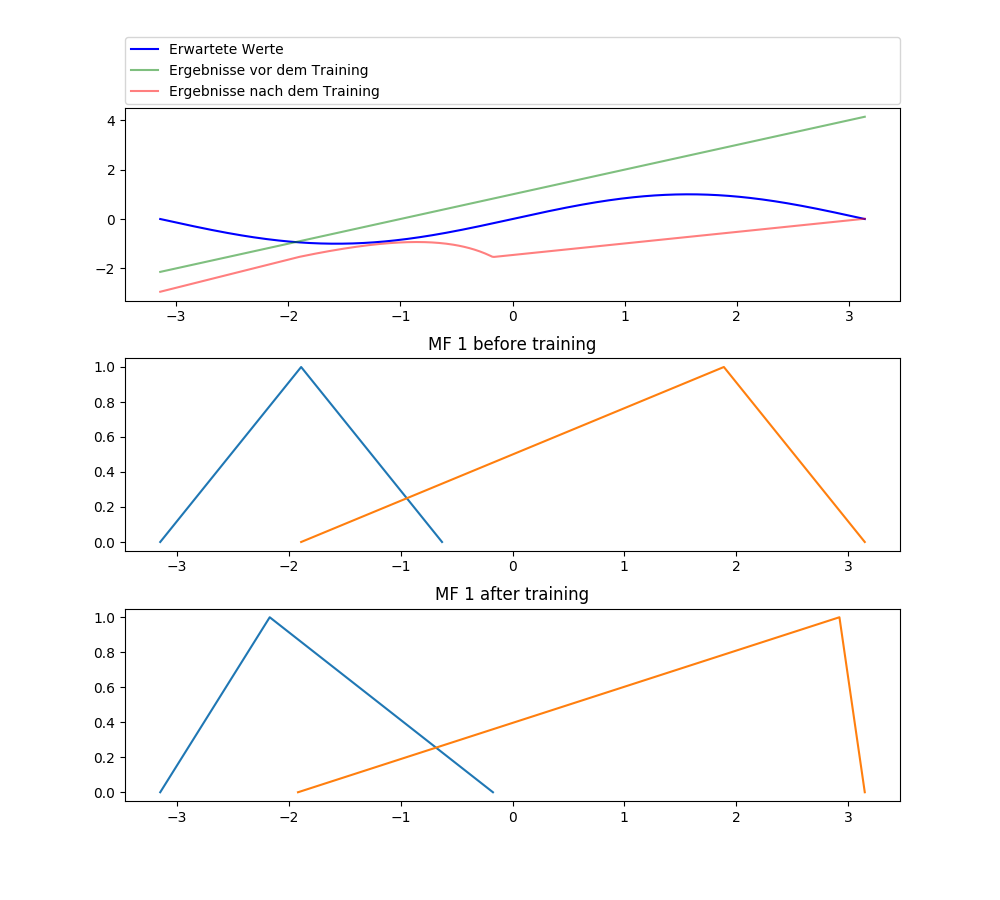
\includegraphics[width=0.65\textwidth]{images/sinus/Stochastic/sinus 1 Input 2 Sets 400 Epochs Stochastic Gradient Descent two equations mf.png}
	\caption{Zwei Fuzzy-Sets, 400 Iterationen, MF-Typ 0} \label{2Sets400_Stoch_0}
\end{figure}



\begin{figure}[htbp]
	\centering
	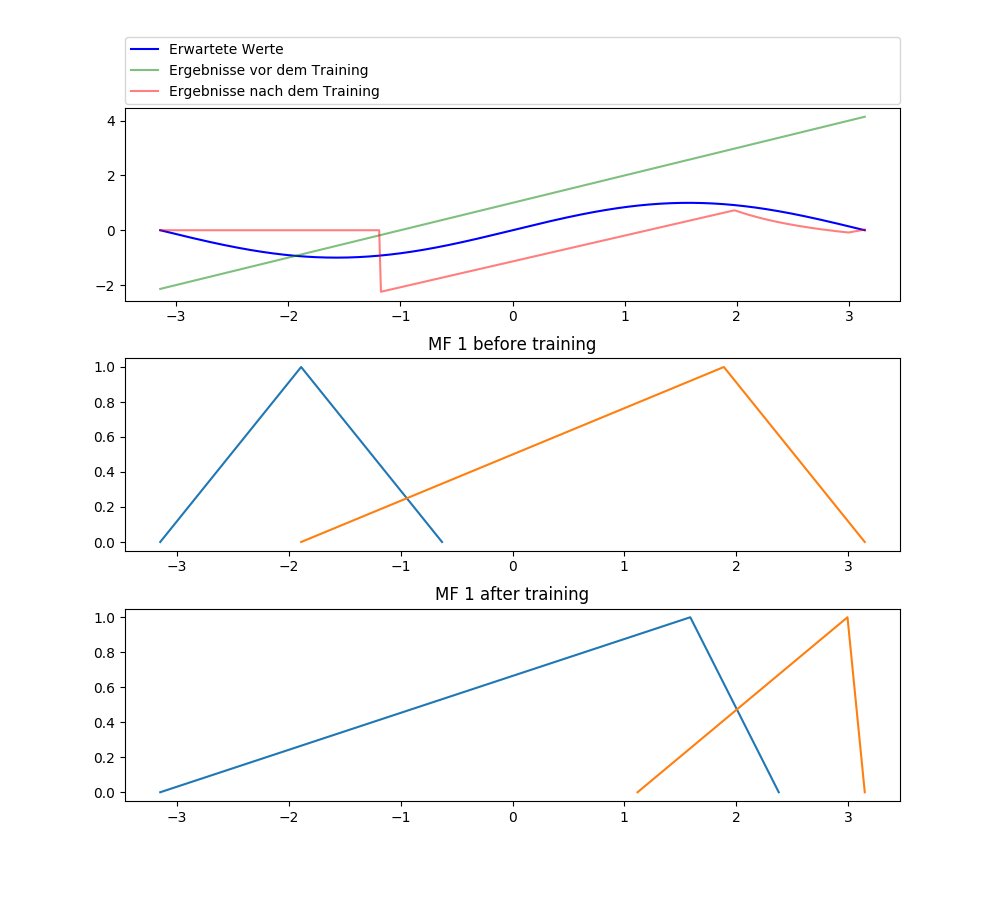
\includegraphics[width=0.65\textwidth]{images/sinus/Stochastic/sinus 1 Input 2 Sets 400 Epochs Stochastic Gradient Descent one equation mf.png}
	\caption{Zwei Fuzzy-Sets, 400 Iterationen, MF-Typ 1} \label{2Sets400_Stoch_1}
\end{figure}

Aus der beiden Abbildungen \ref{2Sets400_Stoch_0} und \ref{2Sets400_Stoch_1} ist es zu bestimmen, dass schon nach einem Lauf große Änderungen zu erkennen sind. In den Abbildungen sind die obersten Grafiken besonders wichtig. Jedoch aus der Abbildung \ref{2Sets400_Stoch_1} ist in der Grafik ein Fehler zu erkennen. Da hat die Funktion im Bereich zwischen -3.2 und -1.2 den 0-Wert. Dieses Fehler scheint weiter in den folgenden Testfällen aufzutauchen, aber verschwindet bei den Mini-Batch- und Batch-Lernverfahren. Interessanterweise erhalten wir zwei unterschiedlichen Endergebnisse, obwohl beide Zugehörigkeitsfunktionen die selbe Funktion berechnen. Man erkennt an den Grafiken weiter, dass die Fuzzy-Sets anders gestalltet sind.

In der Tabelle \ref{tab:2Sets400Epochs} unten ist die Fehlerrate und die Laufzeit abzulesen.

\begin{center}
	\begin{minipage}{\textwidth}
	\begin{tabular}{ | p{3cm} | l | l | p{3cm} | p{3cm} |}
		\hline
		Type & Time & Error & Gradient Type & MF Type \\ \hline
		sinus 1 Input 2 Sets 400 Epochs Stochastic Gradient Descent two equations mf&1.1651129310000004s&1.8500861&Stochastic Gradient Descent&two equations mf
		 \\ \hline
		sinus 1 Input 2 Sets 400 Epochs Stochastic Gradient Descent one equation mf&0.8567342689999995s&0.74594057&Stochastic Gradient Descent&one equation mf
		 \\ \hline
	\end{tabular}
\captionof{table}{Testergebnisse für Modelle mit 2 Fuzzy Sets und 400 Iterationen}\label{tab:2Sets400Epochs}
\end{minipage}
\end{center}

Die interessantesten Spalten aus der Tabelle sind \textit{Time} und \textit{Error}. Die Zahlen deuten, dass MF-Typ 1 die bessere Vorgehensweise sein soll. Jedoch ist das wegen des Fehlers nicht ganz richtig.

Als letztes sind noch die Konklusionsfunktionen der beiden Lernabläufe - Konklusionsfunktionen \ref{mf_0:1} für das Modell mit 2 Sets, 400 Iterationen und MF-Typ 0 und \ref{mf_1:1} für das Modell mit einer Gleichung.

% mf-type 1
%a_0 [[ 0.64128985]
%[-1.45790108]]
%a_y: [[1.14182867]
%[0.46766532]]

% mf-type 2
%a_0 [[-1.14182764]
%[-2.1789615 ]]
%a_y: [[0.94000338]
%[0.35914132]]

\begin{align}
	\begin{split}\label{mf_0:1}
		y_{mft0_1}(x) = 0.64128985 + 1.14182867\cdot x \\
		y_{mft0_2}(x) = -1.45790108 + 0.46766532\cdot x
	\end{split} \\
	\begin{split}\label{mf_1:1}
	y_{mft1_1}(x) = -1.14182764 - 0.94000338\cdot x \\
	y_{mft1_2}(x) = -2.1789615 + 0.35914132\cdot x
	\end{split}	
\end{align}

Aus der Konklusionsfunktionen kann man keine Rückschlüsse ziehen. Die Endkurven sind ähnlich, aber das ist kein Wunder, da beide Modelle versuchen, die selbe Funktion zu lernen. 

\subsubsection{Lernen eines Models mit 2 Fuzzy Sets und 10 Abläufe}\label{m2fs10ab}

Der nächste Test endet in 10 Läufe. Die Zwei Tests zeigen keine positiven Ergebnisse. Die Grafiken für die zwei MF-Typen sind sehr Unterschiedlich. Es werden insgesammt vier Tausend Iterationen pro Test durchgeführt, was etwa 7.3s und 6.9s für MF-Typ-0 und MF-Typ-1 entsprechend dauert. Die Abbildungen \ref{2Sets4000_Stoch_0} und \ref{2Sets4000_Stoch_1} stellen die Ergebnisse der Tests dar.

\begin{figure}[htbp]
	\centering
	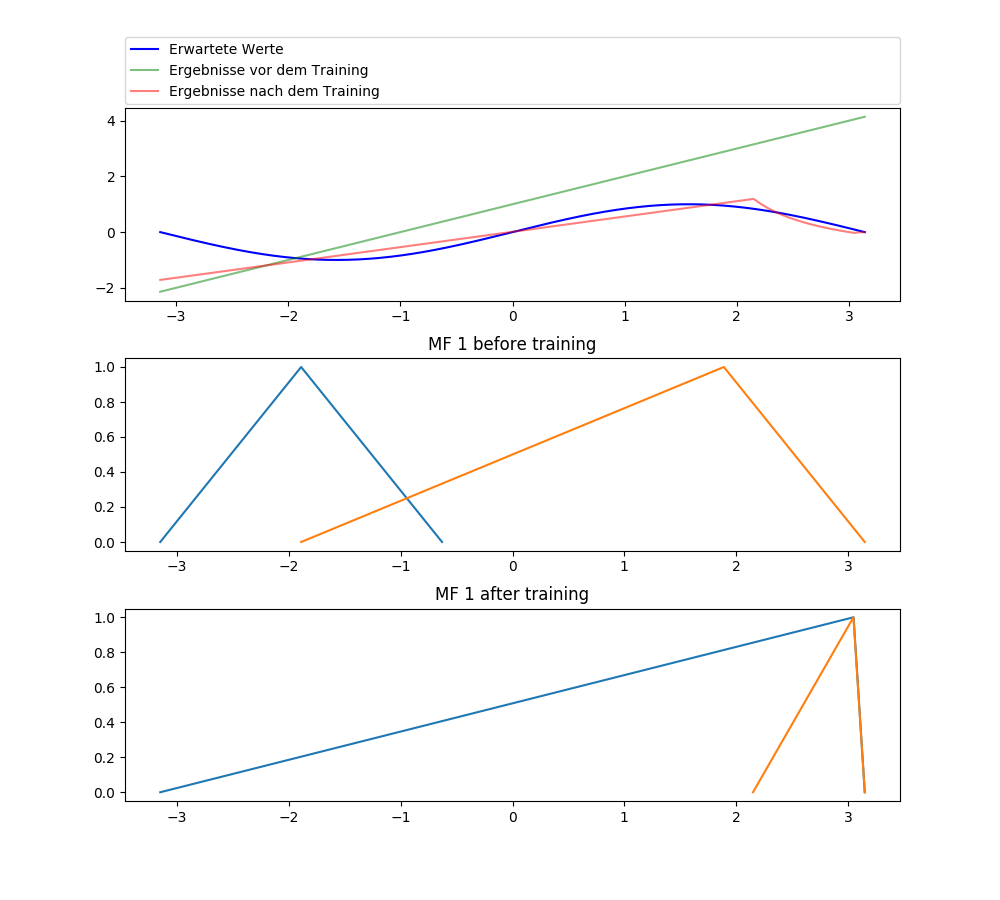
\includegraphics[width=0.65\textwidth]{images/sinus/Stochastic/sinus 1 Input 2 Sets 4000 Epochs Stochastic Gradient Descent two equations mf.png}
	\caption{Zwei Fuzzy-Sets, 4000 Iterationen, MF-Typ 0} \label{2Sets4000_Stoch_0}
\end{figure}
\begin{figure}[htbp]
	\centering
	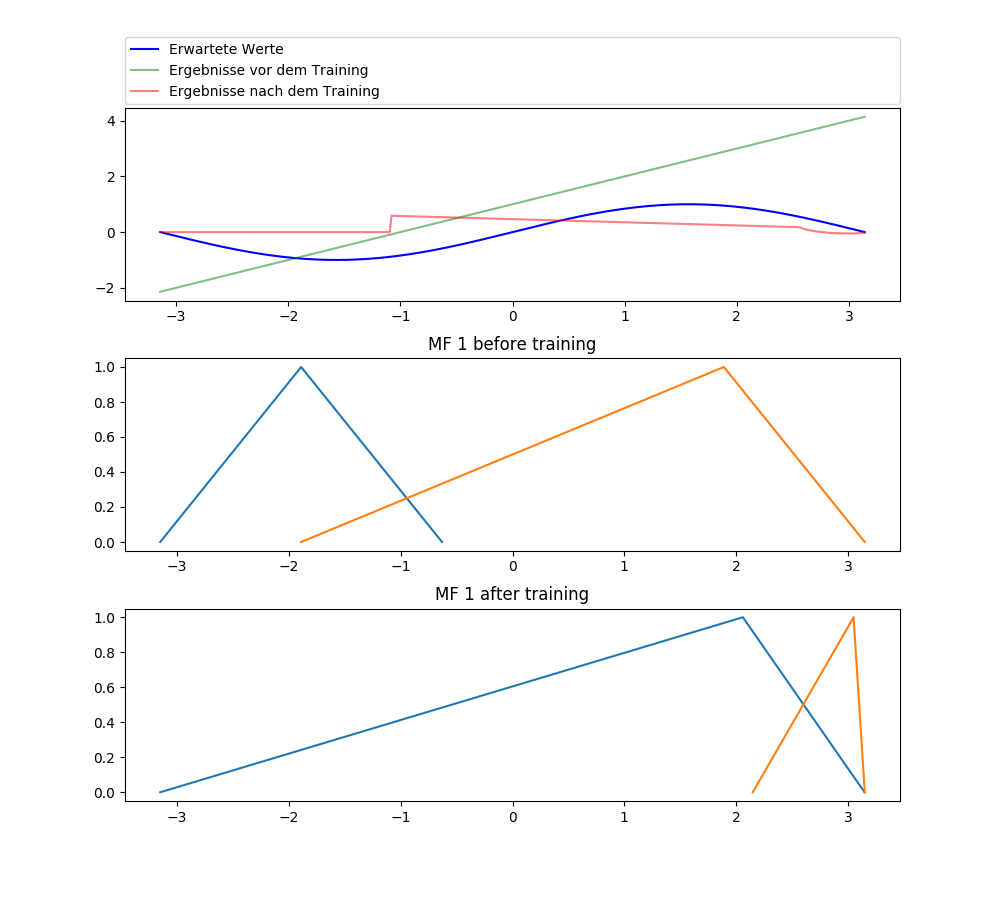
\includegraphics[width=0.65\textwidth]{images/sinus/Stochastic/sinus 1 Input 2 Sets 4000 Epochs Stochastic Gradient Descent one equation mf.png}
	\caption{Zwei Fuzzy-Sets, 4000 Iterationen, MF-Typ 1} \label{2Sets4000_Stoch_1}
\end{figure}

In der Abbildung \ref{2Sets4000_Stoch_1} ist wieder der Fehler in der Berechnung zu bemerken. Der Fehler ergibt sich daraus, dass die Katete der gelbe Zugehörigkeitsfunktion zu lang ist. Was bei kleinen X-Werten dazu führt, dass der rechte Teil der Maximumoperation in der Gleichung \ref{mf_typ1} negativ wird.

Die Konklusionsfunktionen sind für beide Modelle gegeben (\ref{mf_0:10} und \ref{\ref{mf_1:10} sind die Konklusionen entsprechend für die Modelle MF-Typ 0 und MF-Typ 1).
% one equation / MF-Type 0
%a_0 [[ 0.01042824]
%[-1.28822409]]
%a_y: [[ 0.54973926]
%[-0.15157128]]

% one equation / MF-Type 1
%a_0 [[ 0.46553119]
%[-1.52831088]]
%a_y: [[-0.11269253]
%[ 0.44669464]]

\begin{align}
	\begin{split}\label{mf_0:10}
		y_{mft1_1}(x) = 0.01042824 + 0.54973926\cdot x \\
		y_{mft1_2}(x) = -1.28822409 - 0.15157128\cdot x
	\end{split} \\	
	\begin{split}\label{mf_1:10}
		y_{mft2_1}(x) = 0.46553119 - 0.11269253\cdot x \\
		y_{mft2_2}(x) = -1.52831088 + 0.44669464\cdot x
	\end{split}	
\end{align}

Im folgenden Fall gibt es wieder keine Ähnlichkeit zwischen den Konklusionsfunktionen der beiden Modelle.

Die Zeiten und Name als auch die Fehlerrate für beide Modell sind in der Tabelle \ref{tab:2} angegeben. Daraus können zwei Schlüsse gezogen werden.

\begin{center}
	\begin{minipage}{\textwidth}
	\begin{tabular}{ | p{3cm} | l | l | p{3cm} | p{3cm} |}
		\hline
		Type & Time & Error & Gradient Type & MF Type \\ \hline
		sinus 1 Input 2 Sets 4000 Epochs Stochastic Gradient Descent two equations mf&7.308665848s&0.21568511&Stochastic Gradient Descent&two equations mf
		\\ \hline
		sinus 1 Input 2 Sets 4000 Epochs Stochastic Gradient Descent one equation mf&6.9275327529999995s&0.50803167&Stochastic Gradient Descent&one equation mf\\ \hline
	\end{tabular}
\captionof{table}{Testergebnisse für 2 Sets und 4000 Iterationen}\label{tab:2}
\end{minipage}
\end{center}

In der Tabelle können den Fehler und die Laufzeit ausgelesen werden. Anhand der Daten aus dieser Tabelle lässt sich sagen, dass die Berechnung für Modelle des Typs MF-1 kürzer ist, aber das Typ 0 Modell besser lernt.

\subsubsection{Lernen eines Models mit 8 Fuzzy Sets und 10 Abläufe}\label{m8fs10ab}
Im folgenden Testfall ist zu untersuchen, wie die Laufzeit beieinflußt wird, wenn sich die Anzahl der Fuzzymengen erhöht. Im Folgenden Unterkapitel wird der Test mit \textbf{8} Fuzzy-Sets ausgeführt.

Die Ergebnissgrafiken sind zunächst gegeben (\ref{8Sets4000_Stoch_0} und \ref{8Sets4000_Stoch_1}).

\begin{figure}[htbp]
	\centering
	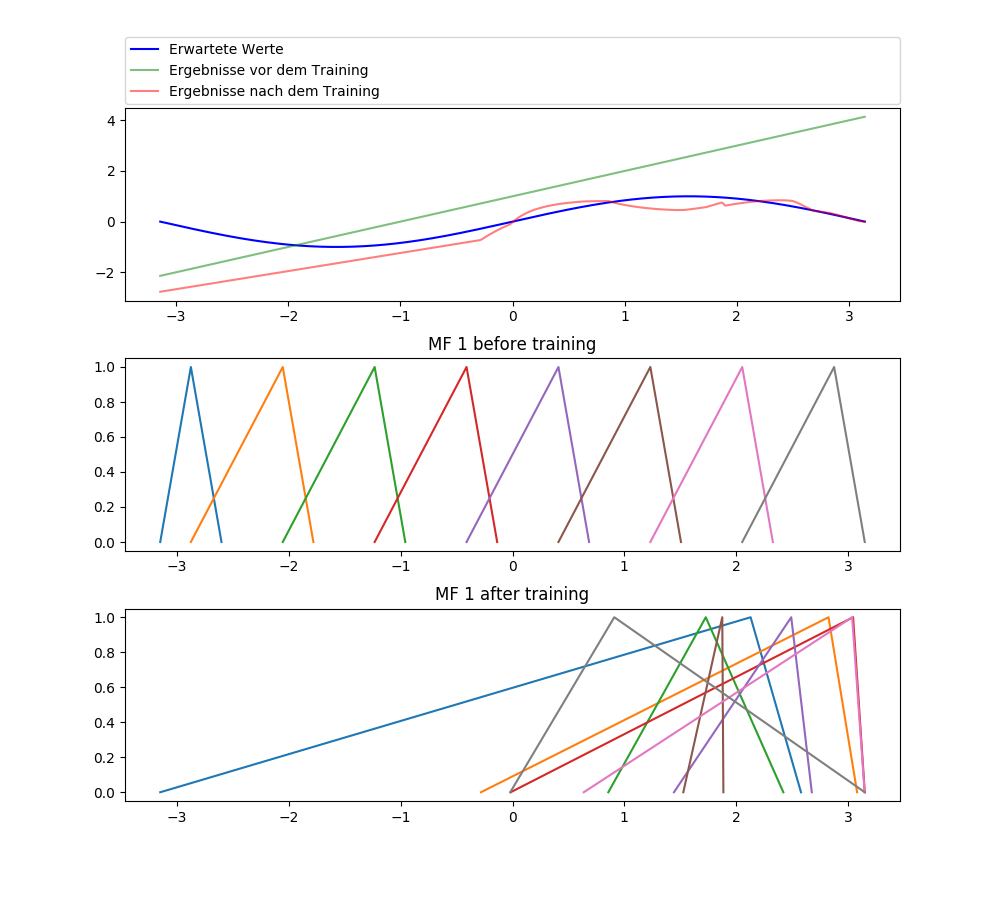
\includegraphics[width=0.65\textwidth]{images/sinus/Stochastic/sinus 1 Input 8 Sets 4000 Epochs Stochastic Gradient Descent two equations mf.png}
	\caption{Acht Fuzzy-Sets, 4000 Iterationen, MF-Typ 0} \label{8Sets4000_Stoch_0}
\end{figure}
\begin{figure}[htbp]
	\centering
	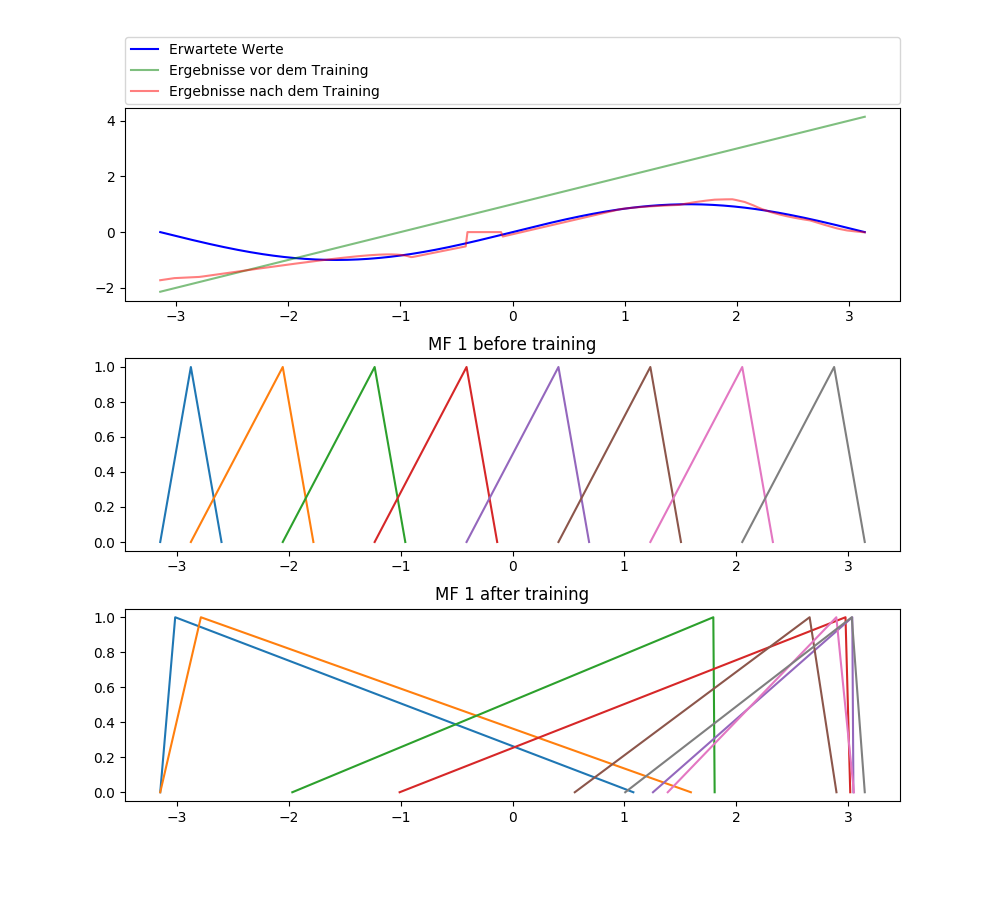
\includegraphics[width=0.65\textwidth]{images/sinus/Stochastic/sinus 1 Input 8 Sets 4000 Epochs Stochastic Gradient Descent one equation mf.png}
	\caption{Acht Fuzzy-Sets, 4000 Iterationen, MF-Typ 1} \label{8Sets4000_Stoch_1}
\end{figure}

An den Abbildugen erkennt man, dass sich die Funktion mit mehr Fuzzy-Mengen besser lernen lässt. Man sieht auch große Unterschiede in der Art der gelernten Fuzzymengen. Es ist zu bemerken, dass alle ab dem zweiten Fuzzyset in der ersten Abbildung in die zweite Hälfte des Wertebereichs vollgestopft werden. Während in der zweite Abbildung ab dem dritten Fuzzyset. Das ist nur deswegen geschehen, weil bei dem Lernen immer Einzelelemente aus der Datenmenge gezogen werden. Üblicherweise werden beim Lernen immer die betroffenen Parametern nach jeder Iteration angepasst. Also die erste Menge wird als erstes angesprochen und angepasst. Da der linke Parameter nicht geändert werden kann, bedeutet das, dass nur der Mittel- und rechten Grenzparameter nach rechts geschoben werden. Dies erklärt die Vollstopfung am rechten Rand des Wertebereichs.

Die Ergebnisse sind in Tabelle \ref{tab8_4000St} abzulesen.

\begin{center}
	\begin{minipage}{\textwidth}
	\begin{tabular}{ | p{3cm} | l | l | p{3cm} | p{3cm} |}
		\hline
		Type & Time & Error & Gradient Type & MF Type \\ \hline
		sinus 1 Input 8 Sets 4000 Epochs Stochastic Gradient Descent two equations mf&17.413568215999998&0.80348945&Stochastic Gradient Descent&two equations mf \\ \hline
		sinus 1 Input 8 Sets 4000 Epochs Stochastic Gradient Descent one equation mf&14.525632421000001&0.21442673&Stochastic Gradient Descent&one equation mf\\ \hline
	\end{tabular}
\captionof{table}{Testergebnisse für 8 Fuzzy-Sets und 4000 Iterationen}\label{tab8_4000St}
\end{minipage}
\end{center}

Aus der Tabelle lässt sich herauslesen, dass der zweite Test (siehe \ref{8Sets4000_Stoch_1}) deutlich schneller und akkurater lernt. Auf der Abbildung \ref{8Sets4000_Stoch_1} ist eine Stuffe im Mittleren Bereich zu erkennen, wo sich der Fehler zeigt. Es ist zu lesen, dass das Typ 1 \textit{3} Sekunden schneller ist. Man sieht auch, dass das Verfahren deutlich näher an dem Sollfunktion ist als Typ 0.

Ich gebe die Konklusionsfunktionen für MF-Typ 0 \ref{8mf_0:10} und MF-Typ 1 \ref{8mf_1:10} nur informative an. Daran können keine weitere Rückschlüsse genannt werden. 
% MF-Typ 0
%a_0 [[-0.5235794 ]
%[ 2.93676464]
%[-3.65265173]
%[ 2.85619127]
%[ 0.1644323 ]
%[-0.92605422]
%[ 0.26038533]
%[ 0.63168423]]
%a_y: [[ 0.71489089]
%[-0.78074253]
%[ 1.63942728]
%[-0.87280814]
%[ 0.55701768]
%[ 1.26660038]
%[-0.12738553]
%[-0.15357252]]
\begin{align}
\begin{split}\label{8mf_0:10}
y_{mft1_1}(x) = -0.5235794 + 0.71489089\cdot x \\
y_{mft1_2}(x) = 2.93676464 - 0.78074253\cdot x \\
y_{mft1_3}(x) = -3.65265173 + 1.63942728\cdot x \\
y_{mft1_4}(x) = 2.85619127 - 0.87280814\cdot x \\
y_{mft1_5}(x) = 0.1644323 + 0.55701768\cdot x \\
y_{mft1_6}(x) = -0.92605422 + 1.26660038\cdot x \\
y_{mft1_7}(x) = 0.26038533 - 0.12738553\cdot x \\
y_{mft1_8}(x) = 0.63168423 - 0.15357252\cdot x
\end{split} \\
% MF-Typ 1
%a_0 [[ 0.46676819]
%[-0.17691342]
%[-0.07739224]
%[ 1.28046489]
%[-1.72202347]
%[ 1.398913  ]
%[ 0.06231506]
%[-0.04088159]]
%a_y: [[ 0.41699012]
%[ 0.80520989]
%[ 0.93785577]
%[-0.94272644]
%[ 0.71823673]
%[ 0.30636544]
%[-0.17987376]
%[-0.28006114]]
\begin{split}\label{8mf_1:10}
y_{mft1_1}(x) = 0.46676819 + 0.41699012\cdot x \\
y_{mft1_2}(x) = -0.17691342 + 0.80520989\cdot x \\
y_{mft1_3}(x) = -0.07739224 + 0.93785577\cdot x \\
y_{mft1_4}(x) = 1.28046489 - 0.94272644\cdot x \\
y_{mft1_5}(x) = -1.72202347 + 0.71823673\cdot x \\
y_{mft1_6}(x) = 1.398913 + 0.30636544\cdot x \\
y_{mft1_7}(x) = 0.06231506 - 0.17987376\cdot x \\
y_{mft1_8}(x) = -0.04088159 - 0.28006114\cdot x
\end{split}	
\end{align}

\subsection{Schlussfolgerung}
Hier ist schwehr die beste Konfiguration fürs Lernen zu nennen. Ich würde sogar sagen, dass das Lernen mit dem stochastischen Verfahren ungeeignet ist. Im nächsten Kapitel wird das Mini-Batch-Verfahren ausgetestet.

Außerdem wird in den nächsten Kapiteln nur auf MF-Typ 0 Modelle konzentriert. Da MF-Typ 1 Modelle nur für symmetrische Fuzzy-Mengen geeignet sind.
%\begin{tabular}
%	
%\end{tabular}
\section{Lernen der Sinusfunktion mit Mini-Batch Gradient Descent}\label{lernen_mb}

In diesem Kapitel handelt es sich um die Mini-Batch Gradient Descent Verfahren. Das Verfahren wurde am Anfang dieses \ref{mini_batch}. Kapitels vorgestellt. Ziel der folgenden Untersuchungen ist es zu zeigen, welche die beste Konfiguration fürs Model ist. Außerdem werden im Fazit die beiden Verfahren (Mini-Batch und Stochastic) verglichen. 

\subsubsection{Lernen der Sinusfunktion mit 2 Fuzzy-Sets und 1 Ablauf}

Begonnen werden soll mit dem Lernen der Funktion mit zwei Fuzzymengen und der Ablauf verläuft über einen Gang. Die Testbeschreibung beinhaltet nur den MF-Typ 0.

\begin{figure}[htbp]
	\centering
	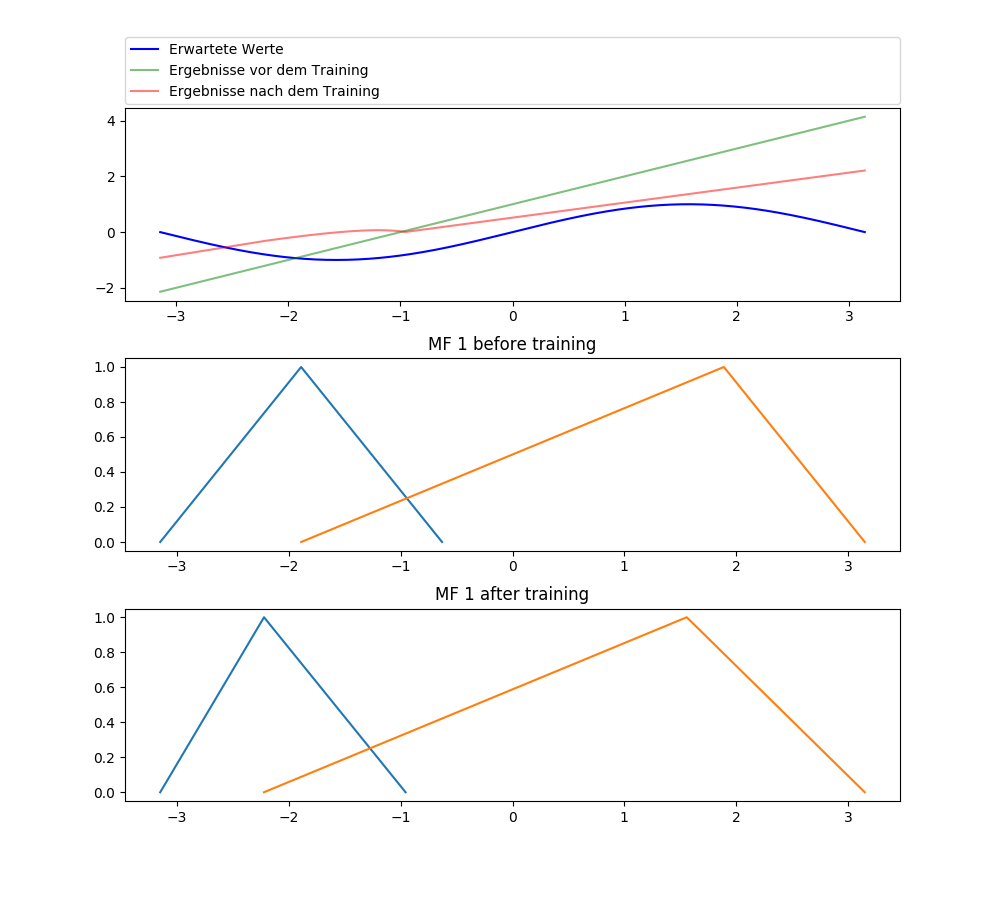
\includegraphics[width=0.75\textwidth]{images/sinus/Mini-Batch/sinus 1 Input 2 Sets 5 Epochs Mini-Batch Gradient Descent two equations mf.png}
	\caption{2 Fuzzy-Sets, 5 Iterationen, MF-Typ 0} \label{2mini_batch5:0}
\end{figure}

In der Abbildung \ref{2mini_batch5:0} sieht man keine große Änderung in den Fuzzy-Sets als auch in der Ergebnissfunktion. Das ist jedoch kein Wunder, da es nur 5 Iterationen durchgeführt werden. Die Dauer dieses Tests entspricht 14 ms.

Zur Abgleich habe ich die Ergebnisse aus dem vorrigen Unterkapitel und diesem Test in der Tabelle \ref{tab2_5MB} angegben.
\begin{center}
	\begin{minipage}{\textwidth}
	\begin{tabular}{ | p{3cm} | l | l | p{3cm} | p{3cm} |}
		\hline
		Type & Time & Error & Gradient Type & MF Type \\ \hline
		sinus 1 Input 2 Sets 5 Epochs Mini-Batch Gradient Descent two equations mf&0.1438041160000001&0.70317644&Mini-Batch Gradient Descent&two equations mf \\ \hline
		sinus 1 Input 2 Sets 400 Epochs Stochastic Gradient Descent two equations mf&1.1651129310000004s&1.8500861&Stochastic Gradient Descent&two equations mf
		\\ \hline
	\end{tabular} 
\captionof{table}{Testergebnisse für Mini-Batch und Stochastic}\label{tab2_5MB}
\end{minipage}
\end{center}

Die Fehlerrate ist wie erwartet sehr hoch, jedoch viel kleiner als der von Stochastischen Verfahren. Außerdem ist die Endfunktion sehr ähnlich wie aus der Vorrigenkapitel (siehe \ref{2Sets400_Stoch_0}). Man erkennt aus den beiden Abbildungen, dass in Abbildung \ref{2Sets400_Stoch_0} die Funktion im Negativen Y-Bereich liegt.%, während die \ref{2mini_batch5:0} nur in dem Abschnit zwischen -3.2 bis ungefähr -1. 

Es ist eine schnellere Laufzeit als der stochastische Verfahren zu erkennen. Die kürze Lerndauer erklärt sich dadurch, da der Datensatz schneller abgearbeitet wird - in Fünf Schritte, im Vergleich zu Vierhundert. Es ist zu erwarten, dass nach 400 Iterationen das Modell noch besser (niedrigere Fehlerrate zu erweisen) sein soll. Im nächsten Kapitel wird diese Aussage untersucht.

Schließlich gebe ich die Konklusionsfunktionen für das Model in \ref{2mini_mf_0:0}.

%MF-Typ 0
%a_0 [[1.12589365]
%[0.51933658]]
%a_y: [[0.65193717]
%[0.53854825]]

\begin{align}
\begin{split}\label{2mini_mf_0:0}
y_{mft1_1}(x) = 1.12589365 + 0.65193717\cdot x \\
y_{mft1_2}(x) = 0.51933658 + 0.53854825\cdot x
\end{split}
\end{align}

Zwischen die Funktionen \ref{2mini_mf_0:0} und \ref{mf_0:1} ist in die Erste Gleichung zu erkennen, dass sich die Parametern ihren Platz getauscht haben. Ein weiterer Unterschied ist, dass es keine negativen Parametern gelernt wurden.

%MF-Typ 1
%a_0 [[0.95071704]
%[0.51425419]]
%a_y: [[0.70936966]
%[0.52004189]]

\subsubsection{Lernen der Sinusfunktion mit 2 Fuzzy-Sets und 10 Ablauf}
Als nächstes ist das Model mit 10 Abläufe zu betrachten. Die Frage, die in diesem Kapitel beantwortet werden soll, ist, ob das Lernen mit einem Bruchteil der Datenmenge wirklich besser ist. Deswegen vergleiche ich die Ergebnisse von Kapitel \ref{m2fs10ab} mit den aus diesem. 

Eine Ergebnissabbildung wird in \ref{2mini_batch50:0} gezeichnet.

\begin{figure}[htbp]
	\centering
	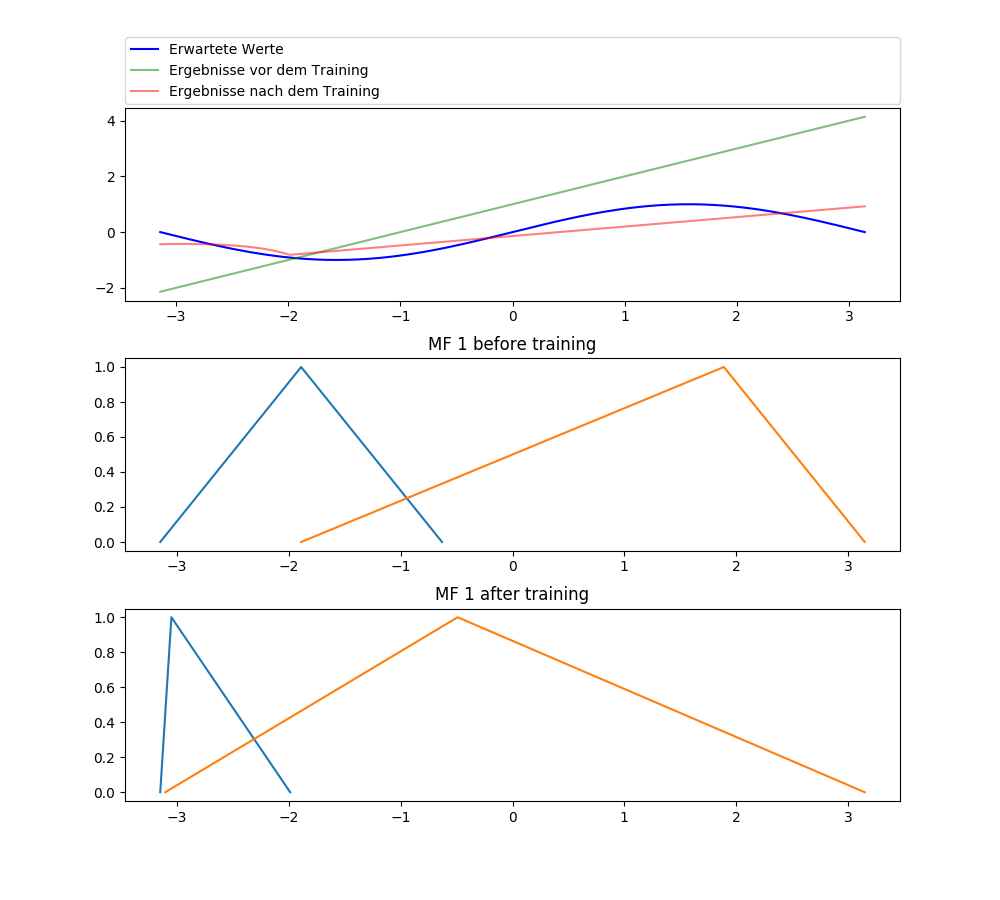
\includegraphics[width=0.65\textwidth]{images/sinus/Mini-Batch/sinus 1 Input 2 Sets 50 Epochs Mini-Batch Gradient Descent two equations mf.png}
	\caption{2 Fuzzy-Sets, 50 Iterationen, MF-Typ 0} \label{2mini_batch50:0}
\end{figure}

Die Fuzzy-Mengen haben eine deutlich größere Änderung im Vergleich zu dem aus vorrigen Kapitel Modell unterlegen. Das Lernen hat 0.2s gedauert. Das ist etwa 30 Mal schneller als der stochastische Verfahren. Die Daten für beide Modelle stehen mit Fehlerrate und Dauer in der Tabelle \ref{tab2_50MB}.

\begin{center}
	\begin{minipage}{\textwidth}
	\begin{tabular}{ | p{3cm} | l | l | p{3cm} | p{3cm} |}
		\hline
		Type & Time & Error & Gradient Type & MF Type \\ \hline
		sinus 1 Input 2 Sets 50 Epochs Mini-Batch Gradient Descent two equations mf&0.2727800499999997&0.1554767&Mini-Batch Gradient Descent&two equations mf\\ \hline
		sinus 1 Input 2 Sets 4000 Epochs Stochastic Gradient Descent two equations mf&7.308665848s&0.21568511&Stochastic Gradient Descent&two equations mf
		\\ \hline
	\end{tabular}  
\captionof{table}{Erbenisvergleich zwischen dem Mini-Batch- und Stochastic-Modell}\label{tab2_50MB}

\end{minipage}
\end{center}

Man erzielt nicht nur ein schnelleres Lernen mit dem Mini-Batch Verfahren,sondern auch ein besseres. Die Fehlerrate ist von 0.22 um etwa 30\% auf 0.16 abgestiegen.

Zum Schluss sind die Inferenzfunktionen \ref{conc_50MB} für das Modell gegeben.

% mftyp 0
%a_0 [[ 0.58986986]
%[-0.14078197]]
%a_y: [[0.32787314]
%[0.3395195 ]]

\begin{align}
\begin{split}\label{conc_50MB}
	y_{mft1_1}(x) = 0.58986986 + 0.32787314\cdot x \\
	y_{mft1_2}(x) = -0.14078197 + 0.3395195\cdot x
\end{split}
\end{align}

\subsubsection{Lernen der Sinusfunktion mit 2 Fuzzy-Sets und 1000 Abläufe}\label{sinus_mb_2_1000}
In diesem Abschnitt wird das Ergebnis aus dem Test mit 1000 Abläufe vorgestellt. Das Model verfügt weiterhin über 2 Fuzzymengen und wird mit MF-Typ 0 gelernt. %Die Abbildung \ref{2mini_batch1000:0} berichtet das Endergebniss.

Bei dieser Konfiguration lernt das Model mit nur einer Zugehörigkeitsgleichung auch sehr erfolgreich. Die Abbildungen der beiden Tests sind sehr ähnlich. Die Abbildungen \ref{2mini_batch1000:1} und \ref{2mini_batch1000:0} berichten das Ergebnis.

\begin{figure}[htbp]
	\centering
	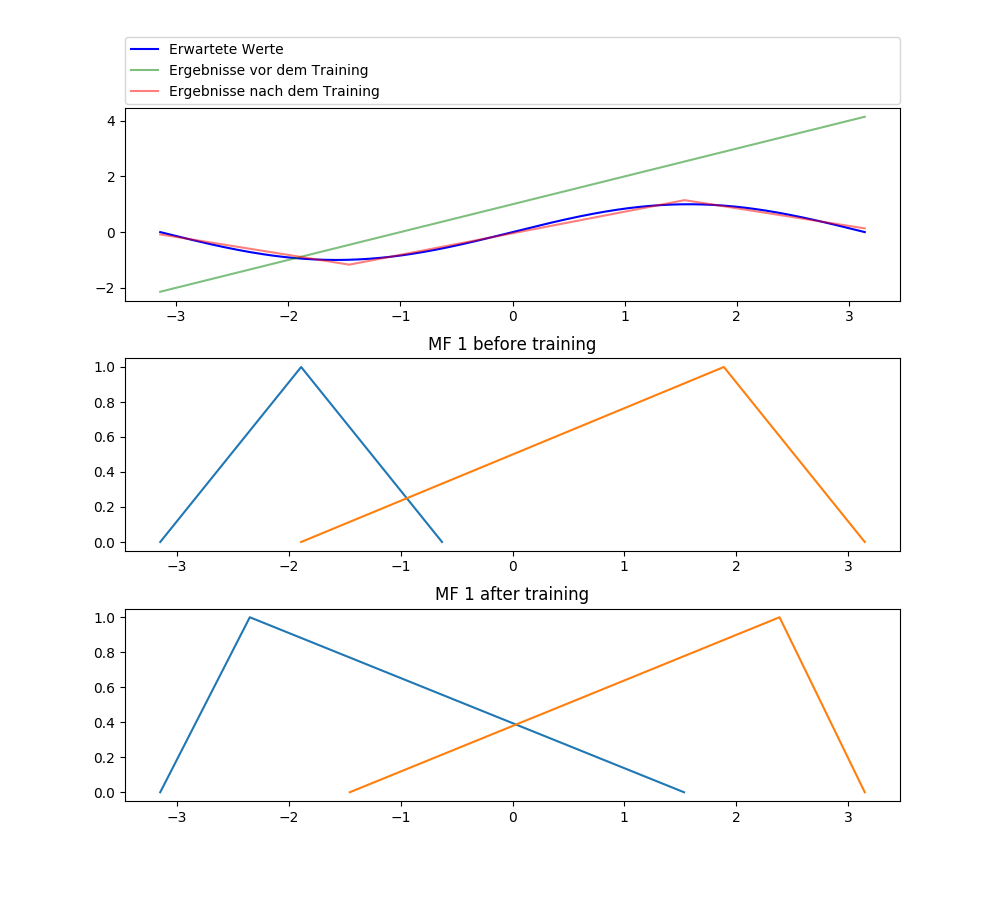
\includegraphics[width=0.65\textwidth]{images/sinus/Mini-Batch/sinus 1 Input 2 Sets 5000 Epochs Mini-Batch Gradient Descent two equations mf.png}
	\caption{2 Fuzzy-Sets, 1000 Iterationen, MF-Typ 0} \label{2mini_batch1000:0}
\end{figure}
\begin{figure}[htbp]
	\centering
	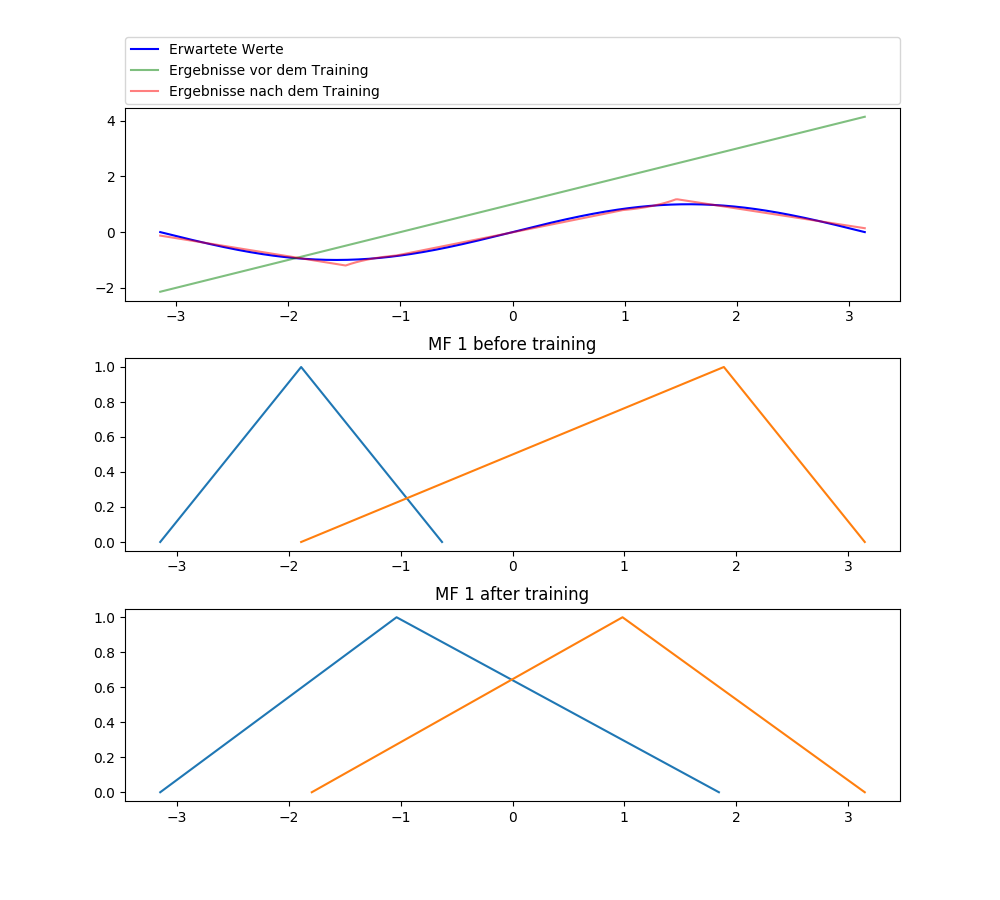
\includegraphics[width=0.65\textwidth]{images/sinus/Mini-Batch/sinus 1 Input 2 Sets 5000 Epochs Mini-Batch Gradient Descent one equation mf.png}
	\caption{2 Fuzzy-Sets, 1000 Iterationen, MF-Typ 0} \label{2mini_batch1000:1}
\end{figure}

Das Endergebnis aus der Abbildung \ref{2mini_batch1000:1} scheint auf den ersten Blick besser zu sein. Der größte Unterschied liegt in den Fuzzymengen. Die gelernten Fuzzysets überlappen zur unterschiedlichen Stuffen. Die Mengen in der Abbildung \ref{2mini_batch1000:1} überschneiden sich deutlich mehr. Die Reichweite ist in der Abbildung \ref{2mini_batch1000:1} etwa 3 cm und auf der Abbildung \ref{2mini_batch1000:0} sind es ungefähr 2. Die zusätzlichen Daten, die in der Tabelle \ref{tab2_1000MB} zu finden sind, beantworten die Frage, welches Model besser ist.

\begin{center}
	\begin{minipage}{\textwidth}
	\begin{tabular}{ | p{3cm} | l | l | p{3cm} | p{3cm} |}
		\hline
		Type & Time & Error & Gradient Type & MF Type \\ \hline
		sinus 1 Input 2 Sets 5000 Epochs Mini-Batch Gradient Descent two equations mf&11.761141329s&0.006521431&Mini-Batch Gradient Descent&two equations mf \\ \hline
		sinus 1 Input 2 Sets 5000 Epochs Mini-Batch Gradient Descent one equation mf&10.697818779s&0.0048954873&Mini-Batch Gradient Descent&one equation mf \\ \hline 
	\end{tabular}
\captionof{table}{Testergebnisse für Modelle mit 2 Sets und 5000 Iterationen}\label{tab2_1000MB}
\end{minipage}
\end{center}

Die Vermutung war richtig. Das zweite Model ist mit etwa 0,02 Einheiten besser und mit einer Sekunde schneller. Die Frage taucht jetzt auf, wo liegt der Unterschied zwischen die beiden Modellen? Ist es wegen des Unterschieds in der Fuzzymengen, oder sind die Inferenzfunktionen einfach unterschiedlich? Die Antwort wird erst klar, wenn die Gleichungen für die Konklusionen betrachtet werden. Analog gehören die ersten beiden Gleichung in \ref{2mf_0:1000} dem Modell mit zwei Gleichungen (MF-Typ 0) und entsprechend \ref{2mf_1:1000} dem Modell mit einer Gleichung (MF-Typ 1).



% Endfunktion mftyp 0
%a_0 [[-2.10781751]
%[ 2.1163349 ]]
%a_y: [[-0.64453965]
%[-0.63109723]]

% Endfunktion mftyp 1
%a_0 [[-2.17036302]
%[ 2.09081218]]
%a_y: [[-0.65073889]
%[-0.62095912]]

\begin{align}
\begin{split}\label{2mf_0:1000}
y_{mft1_1}(x) = -2.10781751 - 0.64453965\cdot x \\
y_{mft1_2}(x) = 2.1163349 - 0.63109723\cdot x
\end{split} \\	
\begin{split}\label{2mf_1:1000}
y_{mft2_1}(x) = -2.17036302 - 0.65073889\cdot x \\
y_{mft2_2}(x) = 2.09081218 - 0.62095912\cdot x
\end{split}	
\end{align}

Die Antwort auf die Frage lautet, dass der Unterschied liegt in den Fuzzymengen. Die Gleichungen sind bis auf der zweiten Dezimalzahl identisch. Die Tatsache, dass die Werte überhaupt so ähnlich sind, ist ein Wunder.

Wenn man die Ergebnisse aus Unterkapitel \ref{lernen_mb} betrachtet, erkennt man wie schlecht das stochastische Verfahren lernt. Allein mit \textbf{10} Abläufe (4000 Iterationsschritte) bei dem Stochastischen-Test (siehe Tabelle \ref{tab:2}) hat man fast die selbe Anzahl an Iterationsschritten (5000) bei dem Mini-Batch-Test (siehe \ref{tab2_1000MB}) und trotzdem ist das Ergebniss \textbf{100} mal schlechter.

\section{Lernen der Sinusfunktion mit Batch Gradient Descent}
Weiterhin werden Modelle erstellt, die das Batch Gradient Descent Verfahren benutzen, um die Sinusfunktion zu erlernen. Jedes Testmodell wird 1000 Abläufe, oder 1000 Iterationen (siehe \ref{batch}), laufen gelassen, aber jedes unterscheidet sich vom nächsten in der Anzahl der Fuzzy-Mengen. Es werden zwei Tests durchgeführt, um zu bestimmen, welche ist die optimale, bzw. ausreichende, Anzahl an Fuzzy-Mengen. Die drei Tests werden entsprechen mit 2 und 3 Fuzzy-Sets trainiert. Außerdem es wird einen Vergleich mit Mini-Batch gezogen. Es ist interessant zu prüfen, ob die beiden Verfahren auch unterschiedliche Ergebnisse erzielen würden.

\subsection{Lernen mit 2 Fuzzy-Sets}\label{lernene_2S_b}
Das erste Testmodelle wird mit 2 Fuzzy-Mengen initialisiert und der Test wird 1000 Abläufe durchgeführt. Das Ergebnis wird in der Abbildung \ref{batch_2_1000} und in der Tabelle \ref{table_2_1000} beschrieben.

\begin{figure}[htbp]
	\centering
	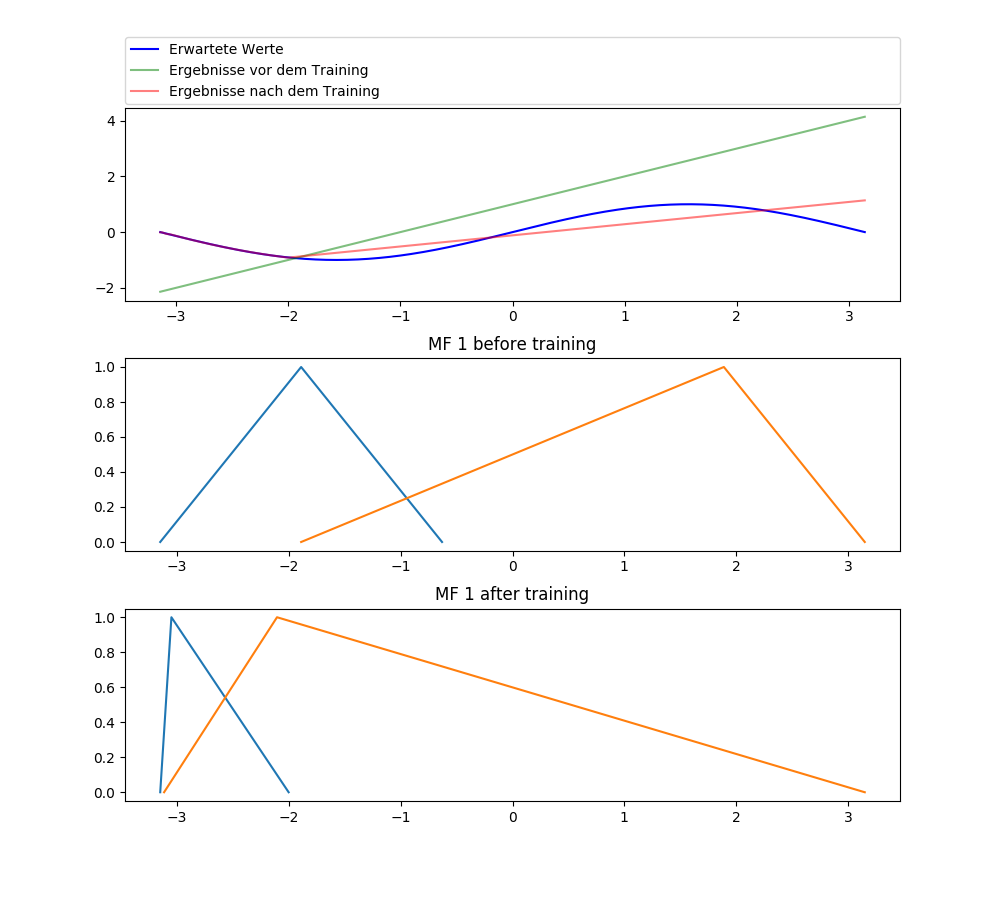
\includegraphics[width=0.65\textwidth]{images/sinus/Batch/sinus 1 Input 2 Sets 1000 Epochs Batch Gradient Descent two equations mf.png}
	\caption{Batch Modell mit 2 Fuzzy-Sets, 1000 Iterationen und MF-Typ 0} \label{batch_2_1000}
\end{figure}

Der Abbildung \ref{batch_2_1000} nach wird in dem Anfangsbereich zwischen den X-Werteb -3.2 und -2.0 scheint die Kurve gut angepasst zu werden. Im späteren Bereich (-2.0 bis 3.2) ist keine Kurve mehr, sondern eine Gerade. Das liegt daran, dass die Fuzzymengen nur zum kleinen Teil überlappen, zwar nur zwischen -3.2 und 2.0, darum auch die anliegende Kurve. Wenn dieses Ergebniss mit dem aus letzen Unterkapitel (siehe \ref{sinus_mb_2_1000}) verglichen wird, sieht man den Unterschied in den Fuzzymengen. Hier schon erkennt man, dass das Mini-Batch-Verfahren geeigneter ist als das Batch. Die Begründung dafür ist, dass mit dem Mini-Batch-Verfahren nach 1000 Abläufe ein gut tranierter Modell erhalten wird. Die Tabelle verschafft uns weitere Information darüber, wie gut das Modell ist.
%


\begin{center}
	\begin{minipage}{\textwidth}
	\begin{tabular}{ | p{3cm} | l | l | p{3cm} | p{3cm} |}
		\hline
		Type & Time & Error & Gradient Type & MF Type \\ \hline
		sinus 1 Input 2 Sets 1000 Epochs Batch Gradient Descent two equations mf&2.1207925870000004&0.13913395&Batch Gradient Descent&two equations mf \\ \hline
		sinus 1 Input 2 Sets 5000 Epochs Mini-Batch Gradient Descent two equations mf&11.761141329s&0.006521431&Mini-Batch Gradient Descent&two equations mf \\ \hline
	\end{tabular}
\captionof{table}{Testergebnisse für die Modelle mit Batch- und Mini-Batch-Verfahren}\label{table_2_1000}
\end{minipage}
\end{center}

Wenn die Zeilen aus der Tabelle \ref{table_2_1000} verglichen wird, erkennt man, dass das Mini-Batch Verfahren besser ist. In der Tabelle kann man lesen, dass es zwei unterschiedliche Werte für die Iterationen der Modelle figurieren. Dies entsteht aus den Unterschieden in der beiden Verfahren (Mini-Batch und Batch). In beiden Testfällen wird 1000 Abläufe durchgeführt, was bei dem Mini-Batch-Modell 5000 Iterationen sind, da einen Ablauf aus fünf Iterationen besteht. Daraus ergibt sich eine natürliche Verzögerung in der Berechnung(dem Lernen). Was aber nicht bestreiten kann ist die Fehlerrate. Hier erweist das Mini-Batch-Modell eine Verbesserung um zwei Stellen nach der Komma.

\subsection{Lernen mit 3 Fuzzy-Sets}
In dieser Unterkapitel wird ein Test mit 3 Fuzzy-Mengen durchgeführt. Das Modell besitzt die selben Eigenschaften wie das aus dem letzen Unterkapitel(siehe \ref{lernene_2S_b}). Analog zur Unterkapitel \ref{lernene_2S_b} wird zuerst eine Abbildung und danach eine Tabelle analysier, jedoch wird jetzt einen Vergleich zwischen dem Modell aus \ref{batch_2_1000} und dem Modell in der Abbildung \ref{batch_3_1000} gezogen. Ziel hier ist es zu prüfen, ob eine Erhöhung der Fuzzy-Sets zum besseren Ergebniss führt. Die Abbildung \ref{batch_3_1000} zeigt das Endergebniss.

\begin{figure}[htbp]
	\centering
	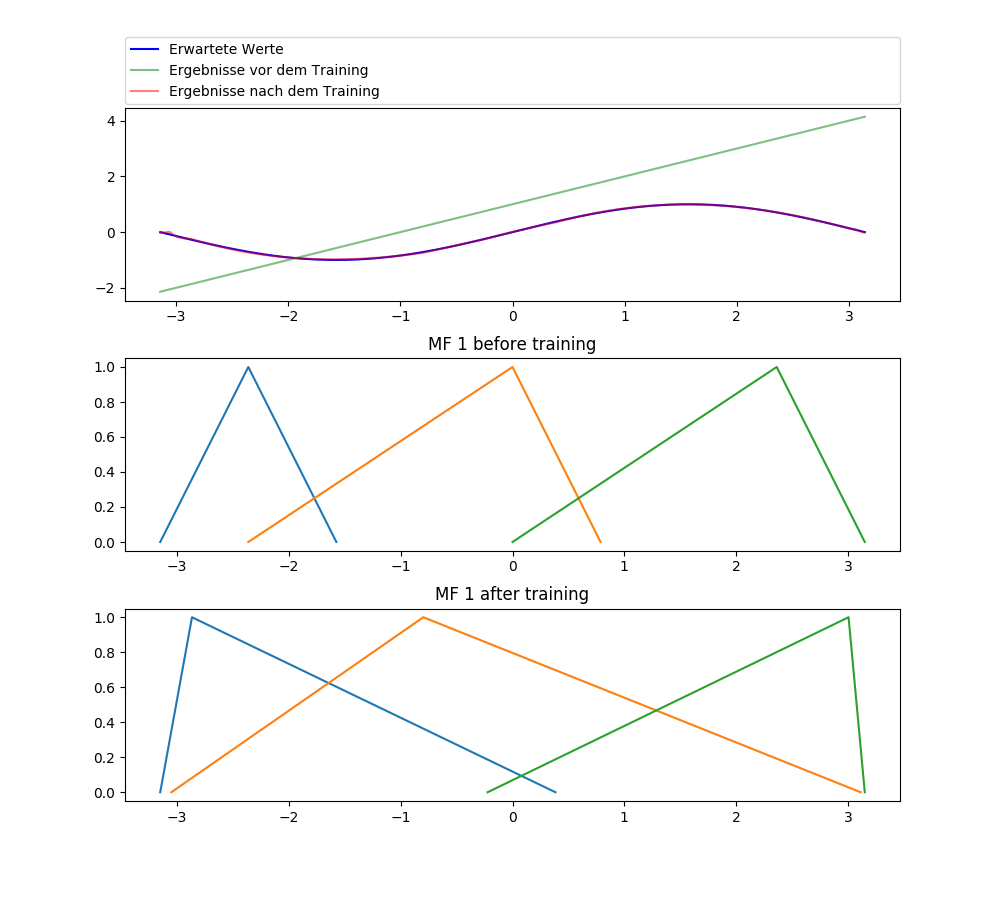
\includegraphics[width=0.65\textwidth]{images/sinus/Batch/sinus 1 Input 3 Sets 1000 Epochs Batch Gradient Descent two equations mf.png}
	\caption{Batch Modell mit 3 Fuzzy-Sets, 1000 Iterationen und MF-Typ 0} \label{batch_3_1000}
\end{figure}

Die Abbildung \ref{batch_3_1000} zeigt eine deutliche Verbesserung in dem, wie die Sinusfunktion gelernt wird. Es kann sogar gesagt werden, dass die Funktion sehr gut gelernt ist. Hier ist es wichtig darauf zu weisen, dass alle drei Fuzzy Mengen zu einem gewissen Teil überlappen. Daraus entsteht auch die fast perfekte Kurve, die die gesuchte Funktion überdeckt.
Weiterhin wird die Tabelle \ref{table_3_1000} untersucht

\begin{center}
	\begin{minipage}{\textwidth}
	\begin{tabular}{ | p{3cm} | l | l | p{3cm} | p{3cm} |}
		\hline
		Type & Time & Error & Gradient Type & MF Type \\ \hline
		sinus 1 Input 2 Sets 1000 Epochs&2.1207925870000004&0.13913395&Batch Gradient Descent&two equations mf \\ \hline
		sinus 1 Input 3 Sets 1000 Epochs&2.528284161&0.00021747834&Batch Gradient Descent&two equations mf
		\\ \hline
		sinus 1 Input 2 Sets 5000 Epochs&11.761141329s&0.006521431&Mini-Batch Gradient Descent&two equations mf \\ \hline
		sinus 1 Input 3 Sets 5000 Epochs&12.479160914&0.00017558844&Mini-Batch Gradient Descent&two equations mf\\ \hline	
	\end{tabular}
	\captionof{table}{Testergebnisse für die Modelle mit zwei und drei Fuzzy-Mengen und Mini-Batch- und Batch-Verfahren}\label{table_3_1000}
\end{minipage}
\end{center}

Die Ausage, die sich aus dem Vergleich der Abbildungen \ref{batch_2_1000} und \ref{batch_3_1000} herausgestellt hat, wird durch die Tabelle \ref{table_3_1000} gestärkt. Was aber wichtiger zu betonen, ist die Verbesserung im Vergleich zu dem Mini-Batch-Verfahren Modell aus Unterkapitel \ref{lernene_2S_b}. Das Endergebniss des drei Set Modells hat sich um etwa einen Dreißigstel verbessert. Außerdem trainiert das Modell schneller und zwar um etwa 5 Mal. Wenn man das Ergebniss in den Zeilen zwei und vier von der Tabelle \ref{table_3_1000} betrachtet, sieht man, dass das Mini-Batch-Verfahren etwas besser lernt, aber langsamer wegen der erhöhten Iterationen ist.

\section{Lernen der Parabelfunktion}

Die Struktur dieser Kapitel ähnelt dem aus Vorherigen. Im Laufe der Ausarbeitung bin ich einer sehr interessanten Frage gestoßen. Ich wollte untersuchen, ob das Vorzeichen der Trainingsdaten einen Einfluß auf das Lernen hat. Um das zu überprüfen, habe ich die Parabelfunktion verändert, so dass die positiven X-Werten einnimmt. In einem der Abschnitte unterscheide ich zwischen die beiden Funktionen.

Die eigentlichen Funktionen, die gelernt werden müssen, sind in zwei Abbildungen \ref{pos_par} und \ref{par} zu sehen:
\begin{figure}
	\begin{minipage}{0.48\textwidth}
		\centering
		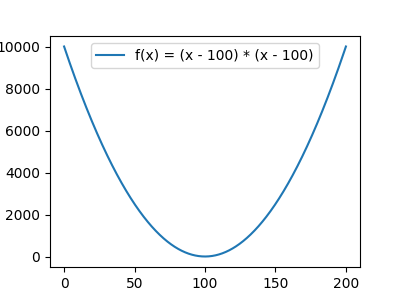
\includegraphics[width=0.65\textwidth]{images/parabola_positive.png}
		\caption{positive Funktion.}
		\label{pos_par}
	\end{minipage} \hfill
	\begin{minipage}{0.48\textwidth}
		\centering
		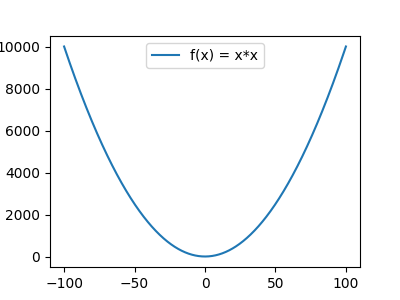
\includegraphics[width=0.65\textwidth]{images/parabola.png}
		\caption{quadratische Funktion.}
		\label{par}
	\end{minipage}
\end{figure}

Auf der ersten Grafik erkennt man, dass die X-Werten nur Positive sind. Ich werde jetzt einige Ergebnisse vorstellen und zeigen, ob die ANFIS-Modelle die Funktionen gleich lernen.

\subsection{Lernen der Parabelfunktion mit Mini-Batch Gradient Descent}

Zuerst betrachten wir zwei Modelle, die das Lernen über 10 Abläufe, bzw. 50 Iterationen, durchführen. Die Ergebnisse sind in den Abbildungen \ref{par_1000_50IT} und \ref{par_pos_1000_50IT} zu lesen.
\begin{figure}[htbp]
	\centering
	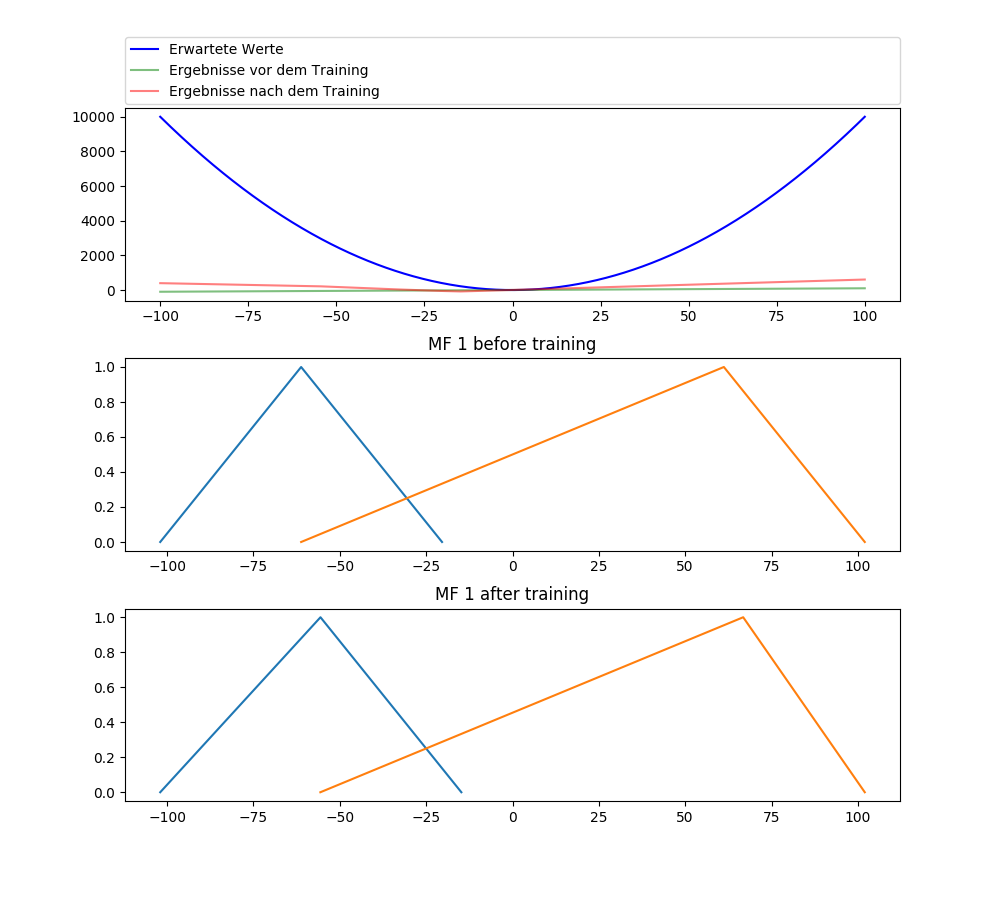
\includegraphics[width=0.65\textwidth]{images/parabola_1000/Mini-Batch/parabola_1000 1 Input 2 Sets 50 Epochs Mini-Batch Gradient Descent two equations mf.png}
	\caption{2 Fuzzy-Sets, 50 Iterationen, MF-Typ 0}
	\label{par_1000_50IT}
\end{figure}
\begin{figure}[htbp]
	\centering
	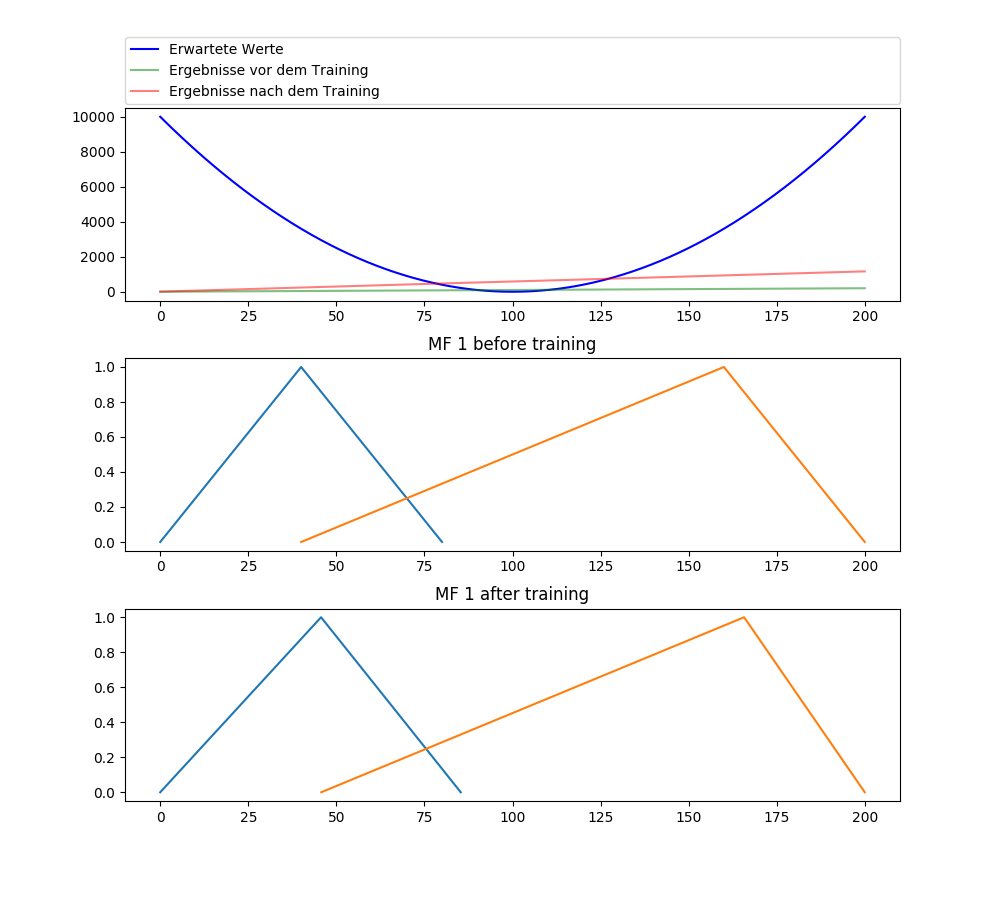
\includegraphics[width=0.65\textwidth]{images/parabola_positive/Mini-Batch/parabola_positive 1 Input 2 Sets 50 Epochs Mini-Batch Gradient Descent two equations mf.png}
	\caption{2 Fuzzy-Sets, 50 Iterationen, MF-Typ 0 mit nur Positiven X-Werte}
	\label{par_pos_1000_50IT}
\end{figure}

In diesem Fall ist die Anzahl der Durchläufe viel zu klein, um wesentliche Ergebnisse geliefert zu werden. Man erkennt, dass in der Grafik \ref{par_1000_50IT} die zwei Enden der Kurve nach oben geschoben sind, während die Mitte auf dem 0-Punkt liegt. In der Grafik \ref{par_pos_1000_50IT} erkennt man keine Kurve wirklich, sondern eine Gerade, welche die selbe wie der Ursprungsgerade ist, aber versetzt. Es werden die nummerische Unterschiede der beiden Modellen in der Tabelle \ref{par_tab1_50MB} betrachtet:

\begin{center}
	\begin{minipage}{\textwidth}
	\begin{tabular}{ | p{3.1cm} | l | l | p{3cm} | p{3cm} |}
		\hline
		Type & Time & Error & Gradient Type & MF Type \\ \hline
		parabola\_1000 & 0.27263559800000037 & 17675046.0 & Mini-Batch Gradient Descent & two equations mf
		 \\ \hline
		parabola\_positive & 0.26520074800000026 & 16615864.0 & Mini-Batch Gradient Descent & two equations mf
		 \\ \hline
	\end{tabular}
\captionof{table}{Testergebnisse für die Modelle}\label{par_tab1_50MB}
\end{minipage}
\end{center} 

Aus der Tebelle \ref{par_tab1_50MB} erkennt man, dass das ``positive'' Modell sowohl schneller als auch ``richtiger'' ist. Die Bilder würden deuten, dass das ``normale'' Model besser ist, aber die nummerischen Daten sagen, dass das andere Modelle das bessere wäre. Das nächste Beipsiel beantwortet die Frage, welche Aufgabe besser gelernt werden kann.

Als nächstes werden wir die zwei Modellen 1000 Mal laufen lassen, das würde heißen das es insgesammt 5000 Iterationen durchgeführt werden. Die weiteren Konfigurationen verbleiben gleich. Zuerst werden die Abbildung \ref{par_5000It} und \ref{par_pos_5000It} aus den beiden Tests gegeben:

\begin{figure}[htbp]
	\begin{minipage}{\textwidth}
	
	\centering
	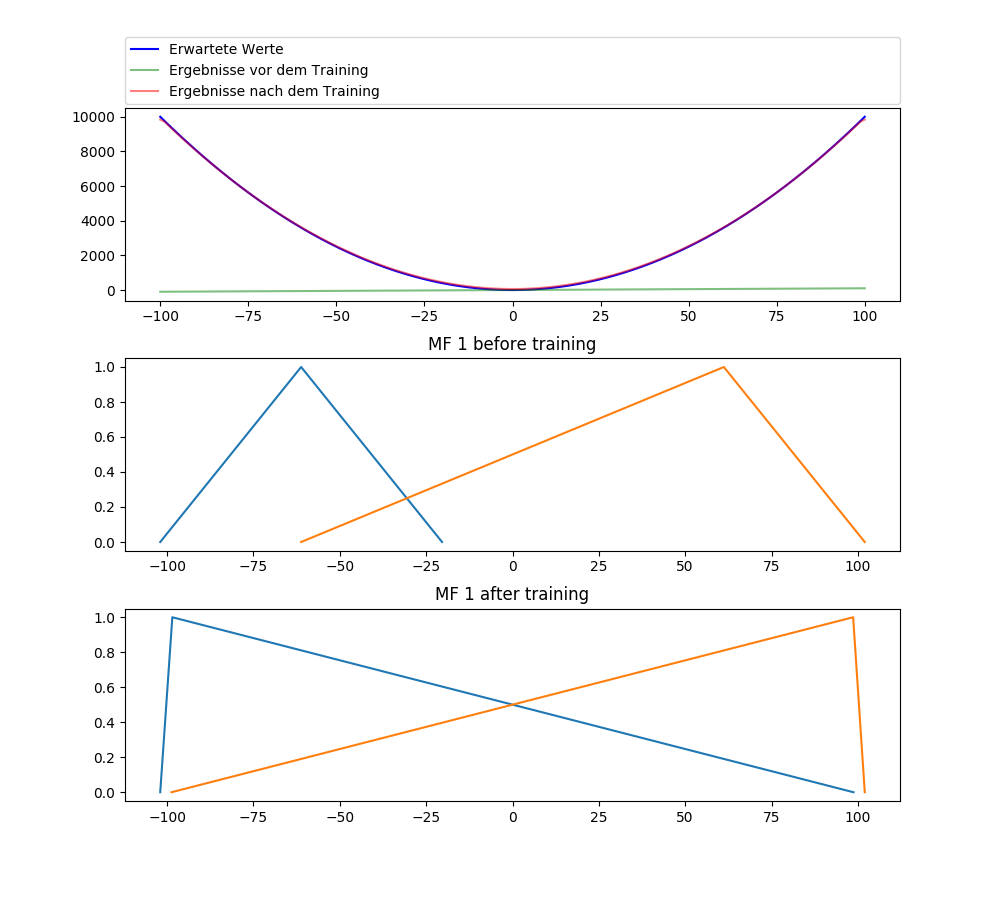
\includegraphics[width=0.65\textwidth]{images/parabola_1000/Mini-Batch/parabola_1000 1 Input 2 Sets 5000 Epochs Mini-Batch Gradient Descent two equations mf.png}
	\caption{2 Fuzzy-Sets, 5000 Iterationen, MF-Typ 0}
	\label{par_5000It}
\end{minipage}
\end{figure}
\begin{figure}[htbp]
	\begin{minipage}{\textwidth}
	
	\centering
	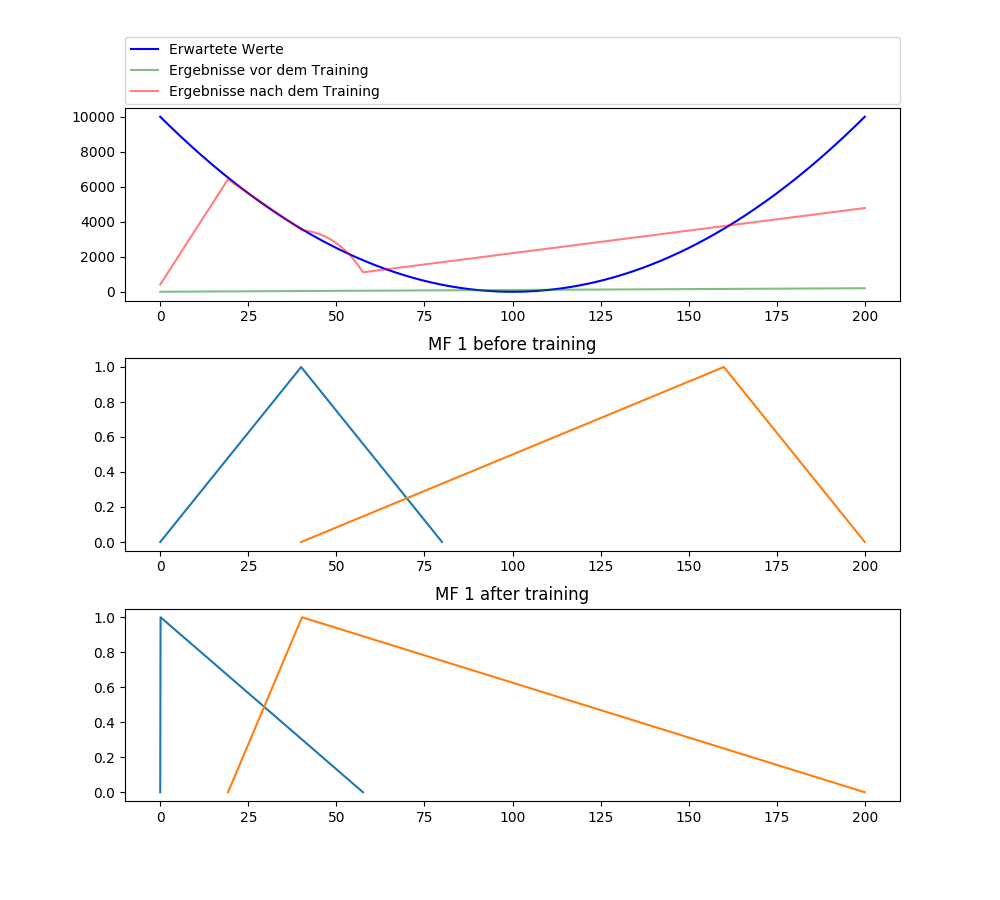
\includegraphics[width=0.65\textwidth]{images/parabola_positive/Mini-Batch/parabola_positive 1 Input 2 Sets 5000 Epochs Mini-Batch Gradient Descent two equations mf.png}
	\caption{2 Fuzzy-Sets, 5000 Iterationen, MF-Typ 0 mit nur Positiven X-Werte}
	\label{par_pos_5000It}
\end{minipage}
\end{figure}

Aus den Abbildungen ist zu lesen, dass das Modell (siehe \ref{par_5000It}) mit positiven und negativen Trainingsdaten schneller den Optimalzustand erreicht als das positve Modell. Außerdem nach 5000 Iterationen ist das Netz sehr gut trainiert. Es ist zu erwarten, dass die nummerische Daten auch für das erste Beispiel sprechen. Die Tabelle \ref{par_tab1_5000MB} beinhaltet die nummerischen Daten.

\begin{center}
	\begin{minipage}{\textwidth}
		
	
	\begin{tabular}{ | p{3.1cm} | l | l | p{3cm} | p{3cm} |}
		\hline
		Type & Time & Error & Gradient Type & MF Type \\ \hline
		parabola\_1000 & 12.538009995&1682.427&Mini-Batch Gradient Descent&two equations mf
		\\ \hline
		parabola\_positive & 12.474743275000002&5956089.5&Mini-Batch Gradient Descent&two equations mf
		\\ \hline
	\end{tabular}
\captionof{table}{Testergebnisee von dem Training der Funktionen ``parabola'' und parabola_``positive''}\label{par_tab1_5000MB}
\end{minipage}
\end{center}

Wie auch schon aus den Grafiken ersichtlich geworden ist, eignet sich das gemischte Modell besser zum lernen. Auch die nummerischen Daten sprechen dafür, dass dies der Fall ist. Es besteht ein riesiger Unterschied in den Fehlerraten der beiden Testfälle.

\section{Fazit}

Die beschriebenen Testfälle wurden explizit ausgewählt, mit dem Ziel bestimmte Eigenschaften nachzuweisen. Der durchgeführten Tests zofolge kann beschlossen werden, dass Modelle mit dem MF-Typ 0 (siehe \ref{mf_typ0}) in meinem Fall geeigneter sind. Das wurde festges aus dem Grund, weil die Berechnung der Zugehörigkeit mit MF-Typ 1 nur für symmetrische Fuzzymengen geeignet ist und der Fehler in den Tests (siehe z.B. Abbildungen \ref{2Sets4000_Stoch_1} und \ref{2Sets400_Stoch_1}) zu erkennen ist. Weiterhin sollte genannt werden, dass der MF-Typ 1 etwas schneller ist, weil er nur eine Berechnung, im Vergleich zu MF-Typ 0, der in zwei Schritten berechnet wird, erfordert.

Es ist sehr wichtig zu erwähnen, dass die Vergrößerung um eine Zusätzliche Menge etwa zwischen 1,2 und 1,3 Mal mehr Laufzeit erfordert. Während einer Verdopplung in Iterationen etwa die doppelte Laufzeit erfordert, was auch zu erwarten ist. Die Abbildung \ref{mini_batch_parabel_grafik} zeigt diese Beziehung.

\begin{figure}[htbp]
	\centering
	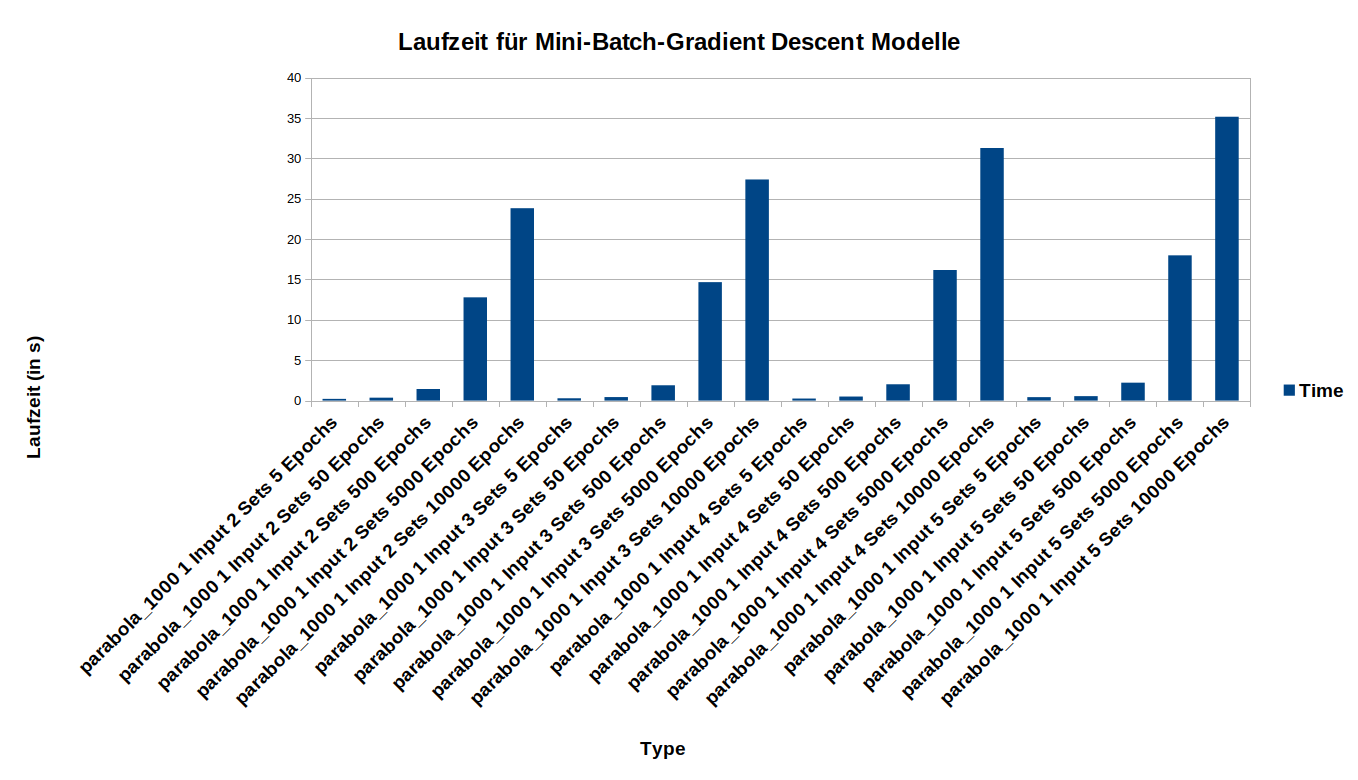
\includegraphics[width=1\textwidth]{images/charts/Mini-BatchGradientTimeParabola_bold.png}
	\caption{Laufzeit für Modelle beim Erlernen der Parabel Funktion}
	\label{mini_batch_parabel_grafik}
\end{figure}

Weiterhin ist es sehr wichtig zu betonen, dass das Lernen mit Mini-Batch und Batch Gradient Descent die bessere Option im vergleich zum Stochastic-Verfahren sind. Einer der Gründe dafür ist, weil es eine bessere Fehlerrate in kleineren Laufzeiten erzielt wird. Diese Behauptung wird durch die nächsten zwei Abbildungen \ref{best_sinus} und \ref{best_parabola}.

\begin{figure}[htbp]
	\centering
	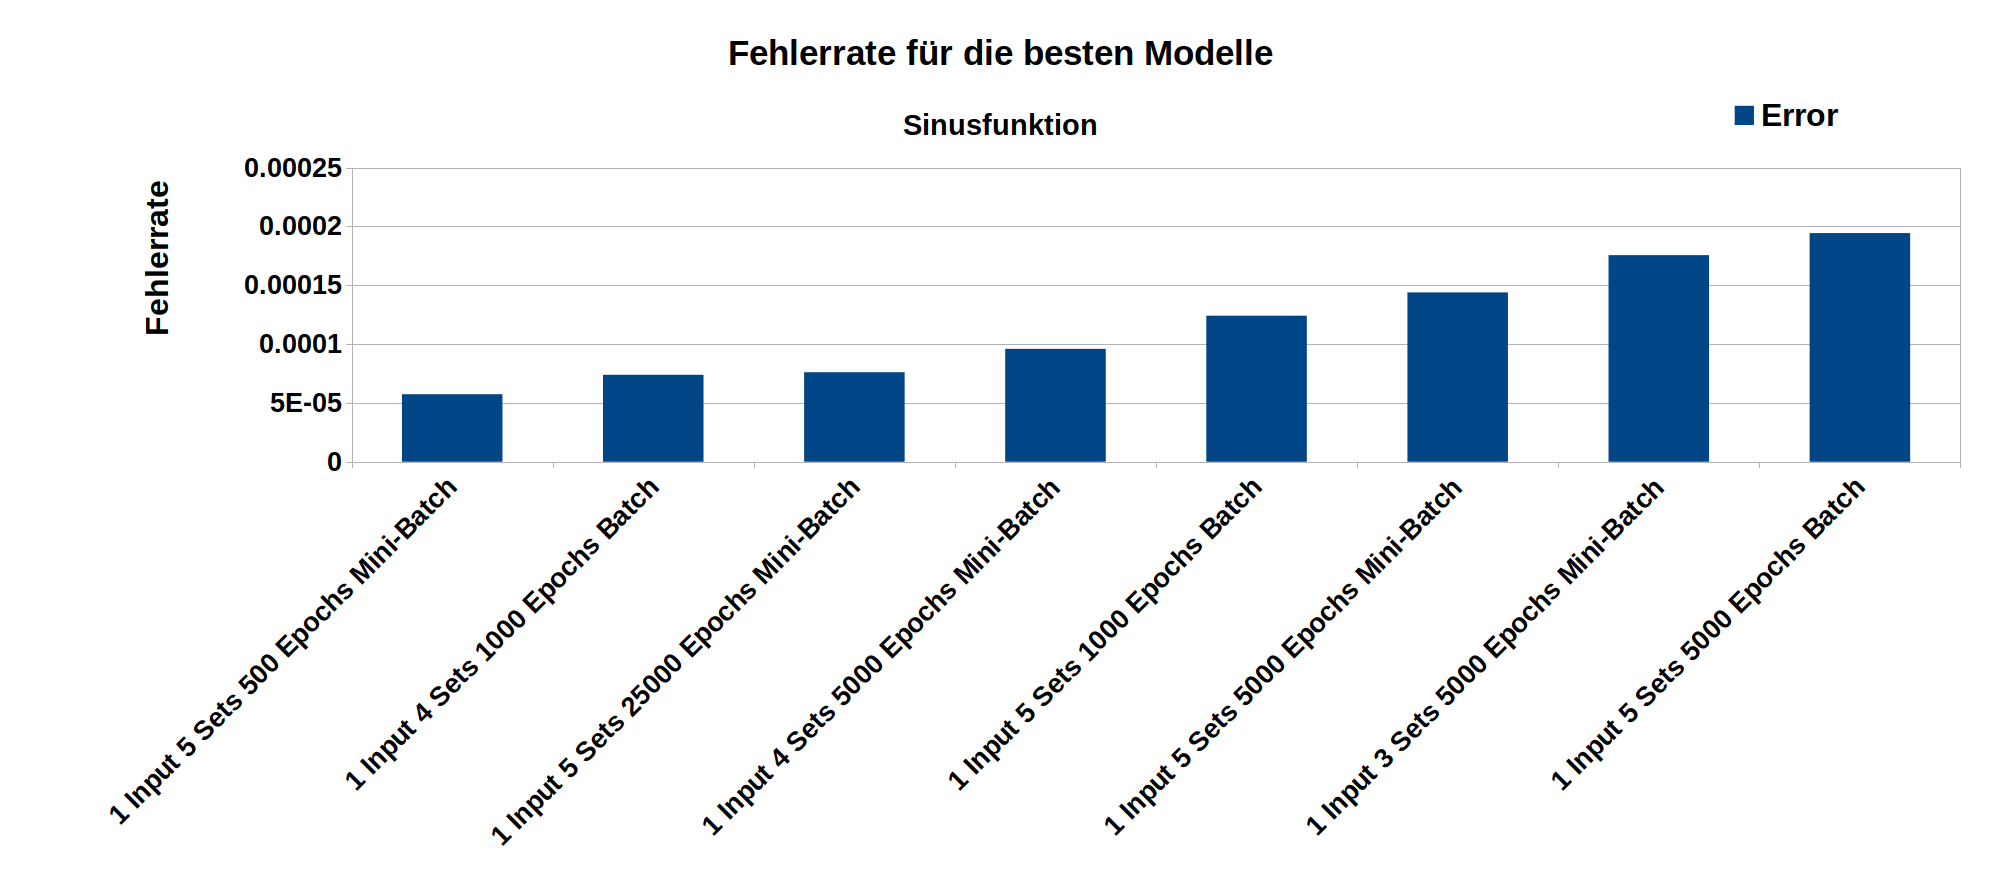
\includegraphics[width=1\textwidth]{images/charts/SinusFunktionbesteModelle_bold.png}
	\caption{Die besten Modelle beim Lernen der Sinusfunktion}
	\label{best_sinus}
\end{figure}

\begin{figure}[htbp]
	\centering
	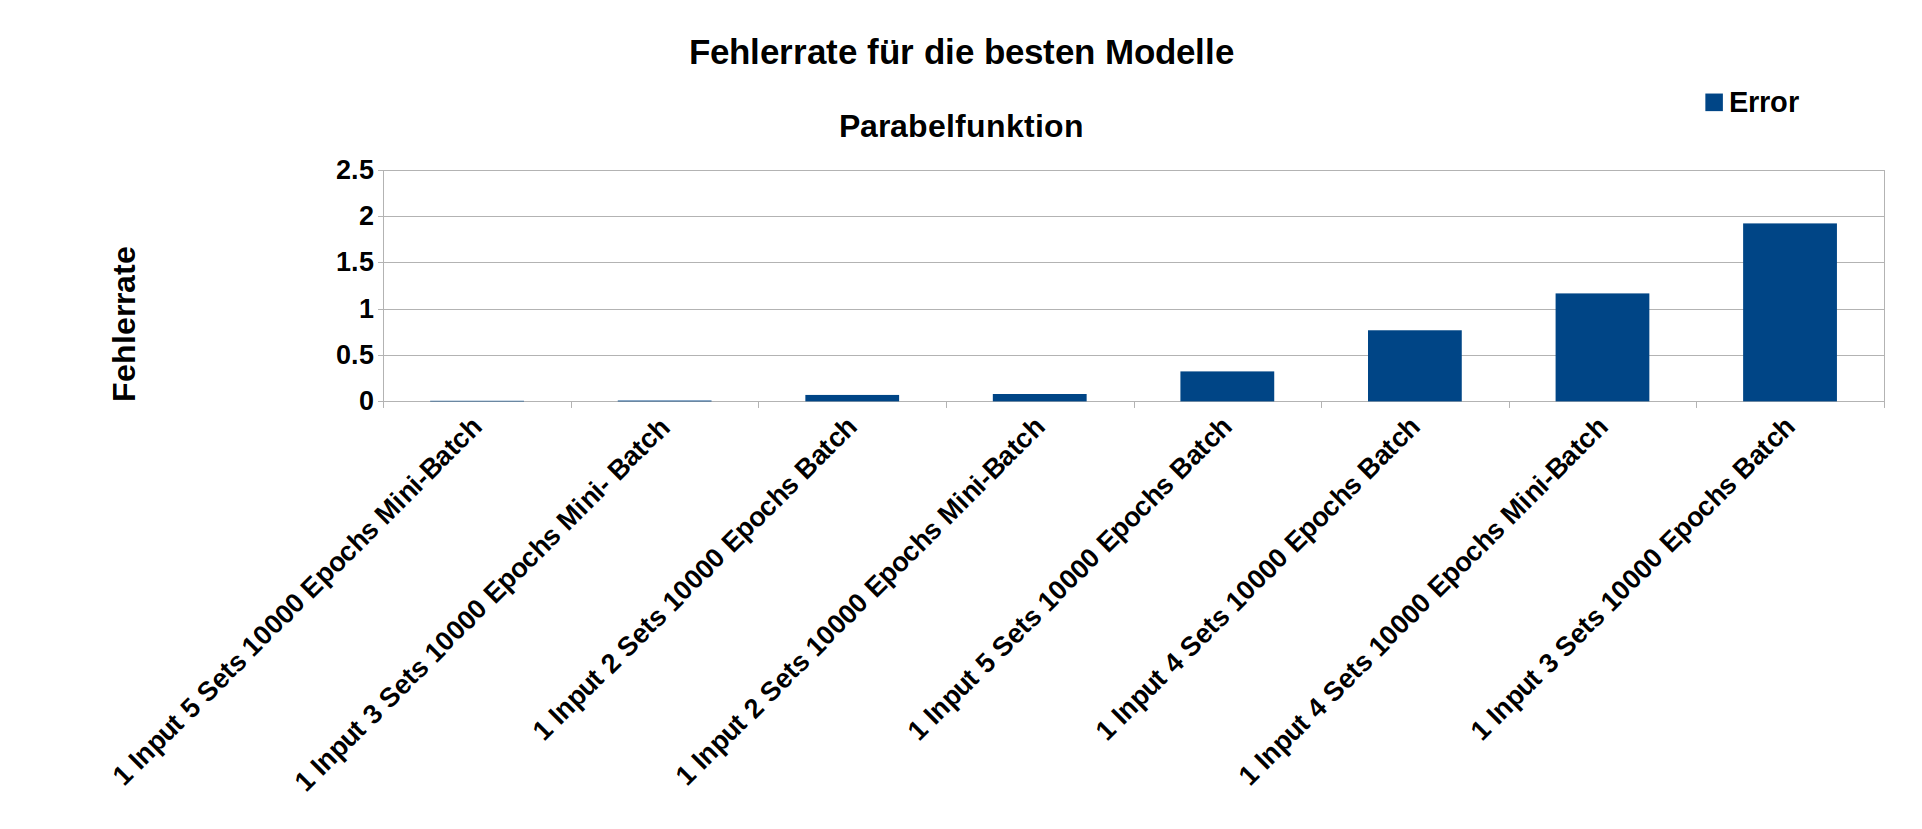
\includegraphics[width=1\textwidth]{images/charts/ParabelFunktionbesteModelle_bold.png}
	\caption{Laufzeit für Modelle beim Erlernen der Parabel Funktion}
	\label{best_parabola}
\end{figure}

Das weitere, was aus den Abbildung \ref{best_sinus} und \ref{best_parabola} zu entnehmen ist, ist, dass der Stochastische Verfahren in keinen der beiden Abbildungen figuriert. Das schließt dieses Verfahren zum Lernen der beiden Funktionen aus.

Aus den beiden Abbildungen \ref{best_sinus} und \ref{best_parabola} kommt man zu der Schlussfolgerung, dass das Mini-Batch-Verfahren bei dem Lernen von beiden Funktionen besser ist. 
%Die Tabelle \ref{best_table} verschafft weitere Informationen dafür, wie die besten Parabel-Modelle in Bezug auf die Laufzeit zueinander im Vergleich stehen.
%
%\begin{center}
%	\begin{minipage}{\textwidth}
%		
%		
%		\begin{tabular}{ | p{3.1cm} | l | l | p{3cm} | p{3cm} |}
%			\hline
%			Type & Time & Error & Gradient Type & MF Type \\ \hline
%			parabola 1 Input 5 Sets 10000 Epochs& 35.160331928& 0.0058110915& Mini-Batch& two equations mf \\ \hline
%			parabola 1 Input 3 Sets 10000 Epochs& 27.390405662& 0.008686484& Mini-Batch& two equations mf \\ \hline
%			parabola 1 Input 2 Sets 10000 Epochs& 22.068964008& 0.06951212& Batch& two equations mf \\ \hline
%			parabola 1 Input 2 Sets 10000 Epochs& 23.82696547& 0.07919865& Mini-Batch& two equations mf \\ \hline
%			parabola 1 Input 5 Sets 10000 Epochs& 36.840694511&  0.32366803& Batch& two equations mf \\ \hline
%			parabola 1 Input 4 Sets 10000 Epochs& 32.4242043& 0.7675758& Batch& two equations mf \\ \hline
%			parabola 1 Input 4 Sets 10000 Epochs& 31.288911103& 1.166094& Mini-Batch& two equations mf \\ \hline
%			parabola 1 Input 3 Sets 10000 Epochs& 27.11144164 & 1.9211318 & Batch&two equations mf \\ \hline
%		\end{tabular}
%		\captionof{table}{Beste Modelle beim Lernen der Parabelfunktion}\label{best_table}
%	\end{minipage}
%\end{center}
%
%Laut der Tabelle \ref{best_parabola} lassen sich keine Schlüsse dafür ziehen, welches Gradienten-Verfahren schneller ist, da in manchen Fällen ist es das Mini-Batch- (Vgl. 1. und 5. Zeile in der Tabelle) und anderen das Batch-Verfahren (Vgl. 2. und 8. Zeile in der Tabelle).  

%Das implementierte von mir Programm unterstützt auch Fuzzy-Systeme mit mehr elementiger Eingabe. Diese Funktionalität wurde jedoch nicht ausführlich getestet und somit auch nicht dokumentiert, weil mein Schwerpunkt in der Untersuchung des Modells lag. Außerdem wurde meine Konzentration auf das Erlernen Neuronaler Netze und genauer Tensorflow gerichtet. Am Ende dieser Arbeitung kann ich für mich sagen, dass ich die genannten Aspekte erfüllt habe und die gesammelten Erfahrungen für mich sehr in der Zukunft sehr wichtig sein werden.


